\documentclass[useAMS,usenatbib]{mn2e}

%_____GENERAL PACKAGES_____
\usepackage{amsmath}	%for \text{} in math mode
\usepackage{amssymb}	%for symbols

%_____FIGURES_____
\usepackage{graphicx}	%for including images
\usepackage{float}	%for [Hhtb] etc of figures
\usepackage{grffile}    %for using underscores in figure filenames
\usepackage{subcaption} %for having sub-captions in figures with multiple panels
\usepackage{placeins} %for \FloatBarrier, which forces all figures to be printed before continuing

%_____SYMBOLS_____
\usepackage{ mathrsfs } %for slanted letters in math mode

%_____FORMAT_____
\setcounter{secnumdepth}{2}	%depth of section numbering
\usepackage{hyperref} %ready-to-lick referencing

%_____MACROS______
\newcommand*\diff{\mathop{}\!\mathrm{d}}
\newcommand*\Diff[1]{\mathop{}\!\mathrm{d^#1}}
%\newcommand{\vect}[1]{\boldsymbol{#1}} % Uncomment for BOLD vectors.
\newcommand{\vect}[1]{\vec{#1}} % Uncomment for ARROW vectors.

%%%%%%%%%%%%%%%%%%%%%%%%%%%%%%%%%%%%%%%%%%%%%%%%

\title[A spiral galaxy's mass distribution uncovered]{A spiral galaxy's mass distribution uncovered through lensing and dynamics}
\author[W. H. Trick, G. van de Ven and A. A. Dutton]{Wilma H. Trick$^{1}$\thanks{E-mail:
trick@mpia.de}, Glenn van de Ven$^{1}$ and Aaron A. Dutton$^{1}$\\
$^{1}$Max-Planck-Institute for Astronomy, K\"{o}nigstuhl 17, 69117 Heidelberg, Germany}
\begin{document}

\date{Accepted [TO DO]. Received [TO DO]; in original form [TO DO]}

\pagerange{\pageref{firstpage}--\pageref{lastpage}} \pubyear{2015}

\maketitle

\label{firstpage}

%--------------------------------------------
%Abstract
\begin{abstract}
We analyse the stellar and dark matter distribution in the spiral galaxy SDSS J1331+3638 (J1331) by means of two independent methods: gravitational lensing and dynamical Jeans modelling. Hubble Space Telescope (HST) imaging by \citet{SWELLSI} show, that J1331's bulge is superimposed by a quadruplet of extended lensing images. By fitting a gravitational potential model to the image positions, we tightly constrain the mass inside the Einstein radius ($R_\text{ein}=0.91\pm0.02$ arcsec) to within 4\% ($M_\text{ein} = (7.8\pm0.3) \cdot 10^{10} M_\odot$). According to the long-slit major axis stellar kinematics from \citet{SWELLSV}, J1331 has a counter-rotating stellar core inside $\sim 2$ arcsec. We model the observed stellar kinematics in J1331's central regions by finding Multi-Gaussian Expansion (MGE) models for the stellar and dark matter distribution that solve the axisymmetric Jeans equations. We find that J1331 requires a steep total mass-to-light ratio gradient in the center to reproduce the observed stellar kinematics. The best fit dynamical model predicts a total mass inside the Einstein radius consistent with the lens model, and vice versa the lens model gives an successful prediction for the observed kinematics in the galaxy center. For a dynamical model including a NFW dark matter halo,  we constrain the halo to have virial velocity $v_{200} \simeq 240 \pm 40$ km/s and a concentration of $c_{200} \simeq 8 \pm 2$ in case of a moderate tangential velocity anisotropy of $\beta_z \simeq −0.4 \pm 0.1$. The NFW halo models can successfully reproduce the signatures of J1331's counter-rotating stellar core and predict J1331's rotation curve at larger radii. However, all these models were more massive than expected from the gas rotation curve and stellar velocity dispersion at larger radii. We speculate that this could indicate a non-trivial re-distribution of matter due a possible minor merger event in J1331's past, e.g. a stellar core in J1331's very center with a \citet{Chabrier2003} initial mass function (IMF), surrounded by a extended stellar bulge population with a super \citet{Salpeter1955} IMF.
\end{abstract}
%--------------------------------------------

\begin{keywords}
blabla -- blabla: bla.
\end{keywords}

%--------------------------------------------
%Introduction
\section{Introduction}

%Intro
Gravitational lensing and dynamical modelling provide independent constraints on the mass distribution of galaxies. Combining them allows for valuable cross-checking opportunities to resolve degeneracies inherent in both methods. It can also help to disentangle the stellar and dark matter content of galaxies, of which the latter is still shrouded by many open questions.\\

%Dark Matter
The flat rotation curves of galaxies (deduced from e.g. the stellar movements in the solar neighbourhood \citep{1932BAN.....6..249O} and $H\alpha$ rotation curves in external galaxies \citep{1978ApJ...225L.107R}) were the first indication that galaxies might reside in massive, almost spherical halos made of invisible ``dark'' matter. The standard model of cosmology, based on results by the Planck Mission \citep{WMAP5cosm}, predicts that $\sim 85\%$ of the universe's total matter content is in the form of non-baryonic cold dark matter. Simulations suggest that this kind of dark matter forms cuspy halos following a Navarro-Frenck-White (NFW) profile \citep{NFW96}. However, central dark matter density cusps are not observed in dark matter dominated dwarf galaxies [TO DO: REF]. If they exist in more massive galaxies depends strongly on stellar mass-to-light ratio [TO DO: REF]. Overall, observations suggest cored dark matter halos. This discrepancy, known as the core-cusp problem, might be due to a yet unknown interaction between dark matter and baryons (e.g. \citealt{2001ApJ...560..636E} [TO DO: more REF]).\\

Determining the overall mass distribution in massive galaxies and separating the dark from the stellar mass components is therefore a crucial step in better understanding the structure of galaxies and nature or dark matter.\\

%Lensing
Strong gravitational lensing is an independent method to tightly constrain the projected total mass of galaxies inside $\sim 1$ arcsec [TO DO: REF]. Massive galaxies can act as gravitational lenses and deflect the light of background sources, giving rise to multiple distorted images of the source [TO DO: REF]. By 2010 over 200 strong gravitational galaxy lenses had been discovered \citep{2010ARA&A..48...87T} and the number is still rising.\\

%Dynamical modelling
The mass profile at larger galactocentric radii can be probed by gas rotation curves that directly measure the galaxy's circlar velocity profile [TO DO: REF]. However, due to its dissipative nature, gas motions are very sensitive to disturbances by e.g. spiral arms and bars [TO DO: REF].\\
Very good and dissipationless dynamical tracers for the underlying gravitational potential are the stars. Their motions are complex, a bulk rotation around one principal axis combined with random motions in all coordinate directions, full dynamical modelling of rotation, dispersion and velocity anisotropies is needed to deduce the matter distribution. An example is axisymmetric Jeans modelling, which solves the Jeans equations for an assumed mass distribution and velocity anisotropy under the assumption of axisymmetry (e.g. \citealt{Cap08}). Degeneracies between stellar and dark matter and velocity anisotropy have to be resolved using additional assumptions.\\
Another dynamical modelling method often applied to external galaxies is e.g. Schwarzschild's orbital superposition approach \citep{schwarzschild}.\\
Because stars are present almost everywhere in the galaxy, stellar dynamical modelling can complement mass constraints from lensing at small and gas motions at large radii.\\

The Sloan WFC Edge-on Late-type Lens Survey (SWELLS, WFC = Wide field camera) \citep{SWELLSI,SWELLSII,SWELLSIII,SWELLSIV,SWELLSV,SWELLSVI} is dedicated to find and investigate spiral galaxies, seen almost edge-on so rotation curves can be easily measured, that are also strong gravitational lenses. By combining lensing and dynamical modelling degeneracies inherent in both methods can be broken. SWELLS picked galaxies in SDSS whose spectra had two different redshifts within 3 arcsec, which makes it likely to capture strong lenses with typical Einstein radii of 1 arcsec. Sufficiently inclined galaxies were picked by eye. Follow up high resolution imaging with the Hubble Space Telescope's (HST) Wide-Field Planetary Camera 2 (WFPC2) was performed to confirm their lensing status \citep{SWELLSI}.\\

%Characteristics of J1331
One of the SWELLS galaxies is SDSS J1331+3638, to which we refer as J1331 in the remainder of this work. It is a spiral galaxy of approximate Hubble type Sb at right ascension = 202.91800$^\circ$ and a declination = 36.46999$^\circ$ (epoch J2000). It has bluish spiral arms and a large reddish bulge (see Figures \ref{fig:F450W} and \ref{fig:F814W}), which is superimposed by quadruplet of extended bluish images approximately at a distance of 1 arcsec from the galaxy center (see Figure \ref{fig:lens_just_imgpos}). The lensed object might be a star-forming blob of a background galaxy. J1331 stands out of the SWELLS sample because of its large counter-rotating core (see Figure \ref{fig:kinematics}), which might be an indication that J1331 underwent a minor merger in its past.\\

%Previous results
\citet{SWELLSI} confirmed that J1331 was a strong gravitational lens, measured its apparent brightness and estimated the stellar masses of disk and bulge. The lensing properties of J1331 were first analysed by \citet{SWELLSIII}. \citet{SWELLSV} measured the gas and stellar kinematics along the major axis and deduced J1331's mass profile from the gas rotation curve at large radii and total mass inside the Einstein radius from gravitational lensing, focusing mostly on the outer regions of J1331.

%Goal of this work
The goal of this work is to complement the previous work on J1331 by an in-depth analysis of the matter distribution in J1331's inner regions. We use stellar dynamical Jeans modelling in addition to lensing constraints, similar to a study of the Einstein Cross by \citet{GlennEC}. We attempt to disentangle the stellar and dark matter components and test if Jeans modelling works also in the presence of a counter-rotating core. Ideally this work on J1331 could also help understanding how minor mergers modify the mass distribution of a galaxy.\\

This paper is organized as follows: Section \ref{sec:Modelling} gives an overview of the modelling techniques used in this work, Section \ref{sec:data} summarizes the data and Section \ref{sec:Results} presents our results on the surface photometry of J1331 using Multi-Gaussian expansions (Section \ref{sec:MGE_results}), constraints from lensing (Section \ref{sec:results_lensing}) and Jeans modelling based on the surface brightness only (Section \ref{sec:results_JAM_SB}) and including a NFW dark matter halo (Section \ref{sec:results_JAM_NFW}). Finally Section \ref{sec:Discussion} uses the result to discuss J1331's stellar mass-to-light ratio and possible merger history and starting points for future work.

%\paragraph{Methods}
%\begin{itemize}
%\item lensing: fitting scale-free galaxy model to image positions \citep{EvansWitt}
%\item photometry: MGE expansion of surface brightness in the F814W filter (deconvolution with PSF), apparent magnitude, total luminosity, effective radius
%\item Jeans modelling: jeans axisymmetric modelling (JAM) by \citet{Cap08} to fit model predictions for the second velocity moments to the stellar kinematics data
%\end{itemize}


%============================================================================


\begin{figure*}
\centering
\begin{subfigure}{.5\textwidth}
  \centering
  \includegraphics[width=.9\linewidth]{fig/first_glimpse_450.ps}
  \caption{J1331 in F450W}
  \label{fig:F450W}
\end{subfigure}%
\begin{subfigure}{.5\textwidth}
  \centering
  \includegraphics[width=.9\linewidth]{fig/first_glimpse_814.ps}
  \caption{J1331 in F814W}
  \label{fig:F814W}
\end{subfigure}
\begin{subfigure}{.5\textwidth}
  \centering
  \includegraphics[width=.9\linewidth]{fig/lens_imgpos.ps}
  \caption{The lensing images}
  \label{fig:lens_just_imgpos}
\end{subfigure}%
\begin{subfigure}{.5\textwidth}
  \centering
  \includegraphics[width=.9\linewidth]{fig/stellar_kinematics_data.ps}
  \caption{Stellar Kinematics by \citet{SWELLSV}}
  \label{fig:kinematics}
\end{subfigure}
\caption{Hubble Space telescope (HST) images and stellar kinematics of the galaxy SDSS J1331+3638 (J1331), which has a large counter-rotating core and whose bulge acts as a strong lens for a bluish background source. \emph{Panel (a) and (b):} HST/WFPC2/WFC3 images of J1331 by \citet{SWELLSI} in two filters, F450W in panel (a) and F814W in panel (b). The galaxy's coordinates on the sky are right ascension $\alpha$ = 202.91800$^\circ$ and declination $\delta$ = 36.46999$^\circ$ (epoch J2000). Image orientation and scaling are indicated in panel (a); the scaling transformation from arcseconds to the physical size of the galaxy in kpc uses the galaxy's redshift $z_d = 0.113$ \citep{SWELLSIII} (i.e. assumes an angular diameter distance of 414 Mpc). The color scaling of these two images is the same. The black solid line in panel (b) shows the orientation of the major-axis. The line has a length of 10 arcsec and indicates the region within which we carry out the Jeans modelling. \emph{Panel (c):} The central region of J1331 in F450W, surface brightness subtracted. An IRAF ellipse [TO DO: How to write and reference????] fit to the F450W surface brightness in panel (a) was subtracted from the image. The (smoothed) residuals within the white square in panel (a) are shown in panel (c). Four bright blobs (A,B,C and D) become visible, which are arranged in a typical strong lensing configuration around the center of the galaxy (G). \emph{Panel (d):} Stellar Kinematics along the galaxy's major axis as measured by \citet{SWELLSV}, line-of-sight rotation velocity $v_\text{rot}$, line-of-sight velocity dispersion $\sigma$ and the rms-velocity $v_\text{rms} = \sqrt{v_\text{rot}^2 + \sigma^2}$. The dotted line in panel (b) indicates the galaxy's effective half-light radius (in the F814W filter), $R_\text{eff} = 2.6" = 5.2$ kpc. The $v_\text{rot}$ curve reveals that J1331 is counter-rotating within $R_\text{eff}$. [TO DO: Add (x,y) axis in figure b).???????]}
\label{fig:specialJ1331}
\end{figure*}
%--------------------------------------------

%------------------------
\section{Modelling} \label{sec:Modelling}
\subsection{Multi-Gaussian Expansion Formalism}

Multi-Gaussian Expansions (MGE) are used to parametrize the observed surface brightness or projected total mass of a galaxy as a sum of $N$ two-dimensional, elliptical Gaussians \citep{1991ApJ...366..599B,1992A&A...253..366M,1994A&A...285..723E,1999MNRAS.303..495E}. This work makes use of the algorithm and code\footnote{Michele Cappellari's IDL code package for fitting MGEs to images is available online at \url{http://www-astro.physics.ox.ac.uk/~mxc/software}. The version from June 2012 was used in this work.} by \citet{Cap02}. We assume all Gaussians to have the same center and position angle $\phi$, i.e. orientation of w.r.t. the $y'$-axis of the coordinate system with polar coordinates $(R',\theta')$ [TO DO: CHECK]. Then the surface brightness can be written as
\begin{eqnarray}
I(R',\theta') &=& \sum_{i=1}^{N} I_{0,i} \exp\left[ - \frac{1}{2\sigma_i^2} \left(x^{'2} + \frac{y^{'2}}{q_i^{'2}}\right)\right]\label{eq:MGEgeneral}\\
\text{with } I_{0,i} &=& \frac{L_i}{2\pi \sigma_i^2 q'_i}\label{eq:centralItotalL}\\
\text{and } x'_i &=& R' \cos(\theta' - \phi)\nonumber\\
y'_i &=& R' \sin(\theta' - \phi),\nonumber
\end{eqnarray}
where $I_{0,i}$ is the central surface brightness of each Gaussian, $L_i$ its total luminosity, $\sigma_i$ its dispersion along the major axis and $q'_i$ the axis ratio between the elliptical Gaussians major and minor axis.
\\We can also expand the telescopes point-spread function (PSF) as a sum of circular Gaussians,
\begin{equation}
\text{PSF}(x,y) = \sum_j \frac{G_j}{2 \pi \delta_j^2} \exp\left[- \frac{1}{2 \delta_j^2} \left(x^2 + y^2 \right)\right], \label{eq:PSFgeneral}
\end{equation}
where $\sum_j G_j = 1$ and $\delta_j$ are in this case the dispersions of the circular PSF Gaussians. In this case the observed surface brightness distribution is a convolution of the intrinsic surface brightness in Eq. (\ref{eq:MGEgeneral}) with the PSF in Eq. (\ref{eq:PSFgeneral}): $(I \ast \text{PSF}) (x',y')$ is then again a sum of Gaussians and can be directly fitted to an image of the galaxy in question.

[TO DO]

\paragraph{Other stuff to mention}
\begin{itemize}
\item [TO DO] analytic deprojection into 3D Gaussians
\end{itemize}


\subsection{Strong gravitational lensing formalism and lens model} \label{sec:lensing_theo}

\paragraph{Lensing formalism.} A gravitational lens is a mass distribution, whose gravitational potential $\Phi$ acts as a lens for light coming from a source positioned somewhere on a plane behind the lens. The angular diameter distance from the observer to the lens is $D_d$, to the source plane it is $D_s$ and the distance between the lens and source plane is $D_{ds}$. The deflection potential of the lens is its potential, projected along the line of sight $z$ and rescaled to
\begin{equation}
\psi(\vect{\theta}) := \frac{D_{ds}}{D_d D_s} \frac{2}{c^2} \int \Phi(\vect{r}=D_d \vect{\theta},z) {\ \mathrm d} z, \label{eq:psidef}
\end{equation}
where $\vect{\theta}$ is a 2-dimensional vector on the plane of the sky. The light from the source at $\vect{\beta} = (\xi,\eta)$\footnote{$\xi$ and $\eta$ are cartesian coordinates on the plane of the sky.} is deflected according to the lens equation
\begin{equation}
\vect{\beta} = \vect{\theta}_i - \left.\vect{\nabla}_\theta \psi(\vect{\theta})\right|_{\vect{\theta}_i} \label{eq:lenseqpot}
\end{equation}
into an image $\vect{\theta}_i = (x_i,y_i)$. The gradient of the deflection potential $\vect{\nabla}_\theta \psi(\vect{\theta})$ is equal to the angle by which the light is deflected multiplied by $D_{ds}/D_{s}$.
\\The total time delay of an deflected light path through $\vect{\theta}$ with respect to the unperturbed light path is given by 
\begin{equation}
\Delta t(\vect{\theta}) = \frac{(1+z_d)}{c} \frac{D_d D_s}{D_{ds}} \left[ \frac 12 (\vect{\theta} - \vect{\beta})^2 - \psi(\vect{\theta})\right], \label{eq:timedelay}
\end{equation}
\citep{BartGravLens}. According to Fermat's principle the image positions will be observed at the extrema of $\Delta t(\vect{\theta})$.
\\The inverse magnification tensor
\begin{equation}
\mathscr{M}^{-1} \equiv \frac{\partial \vect{\beta}}{\partial \vect{\theta}} \overset{(\ref{eq:lenseqpot})}{=} \left(\delta_{ij} - \frac{\partial^2 \psi}{\partial \theta_i \partial \theta_j} \right)\label{eq:magnificationtensor}
\end{equation}
describes how the source position changes with image position. It also describes the distortion of the image shape for an extended source and its magnification due to lensing according to
$$\mu \equiv \frac{\text{image area}}{\text{source area}} = \det \mathscr{M}.$$
Lines in the image plane for which the magnification becomes infinite, i.e. $\det \mathscr{M}^{-1} = 0$, are called \emph{critical curves}. The corresponding lines in the source plane are called \emph{caustics}. The position of the source with respect to the caustic detemines the number of images and their configuration and shape with respect to each other.
\\The \emph{Einstein mass} $M_\text{ein}$ and \emph{Einstein radius} $R_\text{ein}$ are defined via the relation
\begin{equation*}
M_\text{ein} \equiv M_\text{proj}(<R_\text{ein}) \overset{!}{=} \pi \Sigma_\text{crit} R_\text{ein}^2,
\end{equation*}
where $\Sigma_\text{crit} \equiv \frac{c^2}{4\pi G} \frac{D_s}{D_d D_{ds}}$ is the critical density and $M_\text{proj}(<R_\text{ein})$ is the mass projected along the line-of-sight within $R_\text{ein}$. $M_\text{ein}$ is similar to the projected mass within the critical curve $M_\text{crit}$.

\paragraph{Lens model.} Following \citet{EvansWitt} we assume a scale-free model
\begin{equation}
\psi(R',\theta') = R^{'\alpha} F(\theta') \label{eq:scalefreemodel}
\end{equation}
for the lensing potential, consisting of an angular part $F(\theta')$ and a power-law radial part, with $(R',\theta')$ being polar coordinates on the plane of the sky. The case $\alpha = 1$ corresponds to a flat rotation curve. We expand $F(\theta')$ into a Fourier series,
\begin{equation}
F(\theta') = \frac{a_0}{2} + \sum_{k=1}^{\infty} \left(a_k \cos(k\theta') + b_k \sin (k\theta') \right). \label{eq:Fourieransatz}
\end{equation}
For this scale-free lens model the lens equation (\ref{eq:lenseqpot}) becomes
\begin{equation}
\begin{pmatrix} \xi \\ \eta \end{pmatrix} = \begin{pmatrix} R'_i \cos \theta'_i - R_i^{'\alpha-1} \left(\alpha \cos \theta'_i F(\theta'_i) - \sin \theta'_i F'(\theta'_i) \right) \\ R'_i \sin \theta'_i - R_i^{'\alpha-1} \left(\alpha \sin \theta'_i F(\theta'_i + \cos \theta'_i F'(\theta'_i) \right)\end{pmatrix}\label{eq:Fourierlenseq}
\end{equation}
\citep{EvansWitt}, where $F'(\theta') \equiv \partial F(\theta') / \partial \theta'$. When we fix the slope $\alpha$, then the lens equation is a purely linear problem and can be solved numerically for the source position $(\xi,\eta)$ and the Fourier parameters $(a_k,b_k)$ given one observed image at position $(x_i=R'_i \cos \theta'_i,y_i=R'_i \sin \theta'_i)$. 

\paragraph{Model fitting.} As described above our lensing model has the following free parameters: the source position $(\xi,\eta)$, and the radial slope $\alpha$ and Fourier parameters $(a_k,b_k)$ of the lens mass distribution in Equations \ref{eq:scalefreemodel} and \ref{eq:Fourieransatz}. We want to find the lensing model which minimizes for all four images the distance between the observed image positions $\vect{\theta}_{oi}$ and those predicted by the lensing model $\vect{\theta}_{pi}$. Because we want to avoid solving the lens equation (see Equations \ref{eq:lenseqpot} and \ref{eq:Fourierlenseq}) for $\vect{\theta}_{pi}$, we follow \citet{1991ApJ...373..354K} and cast the calculation back to the source plane using the magnification tensor in Equation \ref{eq:magnificationtensor} to approximate $\vect{\theta} \simeq (\partial \vect{\theta} / \partial \vect{\beta}) \vect{\beta} = \mathscr{M} \vect{\beta} $ and the $\chi^2_\text{lens}$ that the fit wants to minimize becomes
\begin{eqnarray*}
\chi^2_\text{lens} &=& \sum_{i=1}^{4} \left|\left( \begin{matrix} \frac{1}{\Delta_x} & 0\\0 & \frac{1}{\Delta_y}\end{matrix}\right) \left( \vect{\theta}_{pi} - \vect{\theta}_{oi} \right)\right|^2\\
&\simeq& \sum_{i=1}^{N} \left|\left( \begin{matrix} \frac{1}{\Delta_x} & 0\\0 & \frac{1}{\Delta_y}\end{matrix}\right)  \left.\mathscr{M}\right|_{\vect{\theta}=\vect{\theta}_{oi}} \left( \begin{matrix} \xi - \tilde{\xi}_i \\ \eta - \tilde{\eta}_i \end{matrix} \right) \right|^2,
\end{eqnarray*}
where $(\Delta_x,\Delta_y)$ are the measurement errors of the image positions $\vect{\theta}_{oi}$. $\left.\mathscr{M}\right|_{\vect{\theta}=\vect{\theta}_{oi}}$ is the magnification tensor and $(\tilde{\xi}_i,\tilde{\eta}_i)$ the source position according to the lens equation, both evaluated at $\vect{\theta}_{oi}$. Following \citet{GlennEC} we add a term
\begin{equation*}
\chi^2_\text{shape} = \lambda \sum_{k \geq 3} \frac{\left(a_k^2 +b_k^2 \right)}{a_0^2} 
\end{equation*}
which forces the shape of the mass distribution to be close to an ellipse. The total $\chi^2$ to minimize is therefore
\begin{equation*}
\chi^2 = \chi^2_\text{lens} + \chi^2_\text{shape}
\end{equation*}
We set $a_1 = b_1 = 0$, which corresponds to the choice of origin; in this case the center of the galaxy.
\\To be able to constrain the slope $\alpha$, we would have needed flux ratios for the images as in \citet{GlennEC}. But the extended quality of the images, possible dust obscuration and surface brightness fluctuations due to microlensing events, as well as the uncertainty in surface brightness subtraction make flux determination too unreliable and we do not include them in the fitting.
\subsection{Jeans Axisymmetric Modelling (JAM)} \label{sec:model_JAM}

Jeans axisymmetric models (JAM) assume galaxies (a) to be collisionless, i.e. the collisionless Boltzmann equation for the distribution function $f(\vect{x},\vect{v},t)$ has to be satisfied ($\frac{\diff f(\vect{x},\vect{v},t}{\diff t} = 0$), (b) in a steady state ($\frac{\partial}{\partial t} = 0$), (c) axisymmetric (best described in cylindrical coordinates $(R,z,\phi)$ and $\frac{\partial}{\partial \phi} = 0$). From this follow the axisymmetric Jeans equations as the vector-valued first moment of the Boltzmann equation, i.e.
\begin{equation*}
\int \frac{\diff f}{\diff t} \Diff3 v = 0.
\end{equation*}
To be able to solve the Jeans equations, additional assumptions about the velocity ellipsoid tensor $\langle v_i v_j\rangle$ have to be made. We follow \citet{Cap08} and assume firstly, that the galaxy's velocity ellipsoid is aligned with the cylindrical coordinate system, i.e. $\langle v_i v_j\rangle = 0$ for $i\neq j$. Secondly, we assume a constant ratio between the radial and vertical 2nd velocity moments, $\beta_z \equiv 1 - \langle v_z^2 \rangle / \langle v_R^2\rangle$. This reduces the Jeans equations to two equations for $\langle v_z^2 \rangle$ and $\langle v_\phi^2 \rangle$, that can be solved by means of one integration,
\begin{eqnarray*}
n \langle v_z^2 \rangle (R,z) &=& \int_0^\infty n \frac{\partial \Phi}{\partial z} \diff z\\
n \langle v_\phi^2 \rangle (R,z) &=& R \frac{\partial}{\partial R} \left( \frac{n \langle v_z^2 \rangle}{1-\beta_z} \right) + \frac{n \langle v_z^2 \rangle}{1 - \beta_z} + R n \frac{\partial \Phi}{\partial R},
\end{eqnarray*}
where $n(\vect{x}) = \int f(\vect{x},\vect{v}) \diff3 v$ is the number density of tracers and $\Phi(\vect{x})$ the galaxy's gravitational potential, generated by the mass density $\rho(\vect{x})$ via Poisson's equation.
\\The JAM modelling approach by \citet{Cap08} makes use of expressing the tracer density and the mass density as MGEs (see also \citet{1994A&A...285..723E}). The density of stellar tracers is assumed to be proportional to the observed and deprojected brightness distribution $\nu(R,z)$ in Eq. (\ref{eq:deprojMGE}). The mass density consists of several sets of MGEs: One MGE, that is usually taken to be $\nu(R,z)$ multiplied by a constant stellar mass-to-light ratio $\Upsilon_*$, describes the distribution of stellar mass in the galaxy. To mimick gradients of stellar mass-to-light ratio, each Gaussian could be assigned its own $\Upsilon_{*,i}$. To add a Navarro-Frenck-White (NFW) \citep{Navarro+1995c,NFW96} dark matter halo component, a MGE generated from a fit to a NFW profile can be added to the stellar component. [TO DO: continue on p. 74] 


\paragraph{Data comparison.} As data we use stellar line-of-sight rotation velocities $v_\text{rot} \equiv \langle v_\text{los} \rangle$ [TO DO: consistent, los or rot] and velocity dispersions $\sigma$ as described in \S\ref{sec:data}. The JAM models give us a prediction for the second line-of-sight velocity moment $v_\text{los}$. The root mean square (rms) line-of-sight velocity $v_\text{rms}$ allows a data-model comparison by relating theses velocities according to 
\begin{equation*}
v_\text{rms}^2 = \langle v_\text{los}^2 \rangle = v_\text{rot}^2 + \sigma^2.
\end{equation*}
The model in Eq. [TO DO] predicts the intrinsic $\langle v_\text{los}^2 \rangle$ at a given position on the sky, which have then to be modified to model the mode of observation, to be comparable to the measurements. The measured $v_\text{rms}$ is a light-weighted mean for a pixel along the long-slit of the spectrograph, with height $L_y = 1$ arcsec \citep{SWELLSV} and a certain given extent in along the major axis, $L_x$, i.e. for a rectangular aperture
\begin{equation*}
\text{AP}(x,y) = \left\{ \begin{array}{ll} 1 & \text{for } -\frac{L_x}{2} \leq x \leq + \frac{L_x}{2} \text{ and } - \frac{L_y}{2} \leq y \leq + \frac{L_y}{2}  \\ 0 & \text{otherwise} \end{array} \right. .
\end{equation*}
The light arriving at the spectrograph itself was subject to seeing, i.e. a Gaussian 
\begin{equation*}
\text{PSF}(x,y)=\mathscr{N}(0,FWHM/2\sqrt{2\ln2})
\end{equation*}
with FWHM=1.1 arcsec  \citep{SWELLSV}. The model predictions have therefore to be convolved with the convolution kernel
\begin{eqnarray*}
K(x,y) &=& (\text{PSF} \ast \text{AP})(x,y) \\
&=& \frac{1}{4} \prod_{u \in \{x,y\}} \left[ \text{erf}\left( \frac{L_u/2 - u}{\sqrt{2}\sigma_\text{seeing}}\right) + \text{erf} \left( \frac{L_u/2 + u}{\sqrt{2} \sigma_\text{seeing}} \right) \right]
\end{eqnarray*}
and weighted by the surface brightness $I(x,y)$ [TO DO: primed x and y or not????]
\begin{eqnarray*}
I_\text{obs} &=& I \ast K\\
\langle v_\text{los}^2 \rangle |_\text{obs} &=& \frac{(I \langle v_\text{los}^2\rangle) \ast K}{I_\text{obs}}.
\end{eqnarray*}
If provided with with the convolution kernel, the JAM code by \citet{Cap08} [TO DO: reference code] performs the convolution numerically. We set $L_x = 0.21$ arcsec as the width of the model pixel, and get a prediction for the actual measurements in bins of width 0.63, 1.26 and 1.89 arcsec \citep{SWELLSV} as light-weighted mean from each 3, 6 and 9 model pixels.

\paragraph{Rotation curve.} The intrinsic rotation curve is the first velocity moment $\langle v_\phi\rangle = \sqrt{\langle v_\phi^2 \rangle - \sigma_\phi^2}$. The observed rotation curve is the projection of the light-weighted contributions to $\langle v_\phi\rangle$ along the line-of-sight(\cite{Cap08}),
\begin{equation*}
I \langle v_\text{los}\rangle = \int_{-\infty}^{+\infty} \nu \langle v_\phi\rangle \cos \phi \sin i \diff z'.
\end{equation*}
The first velocity moments cannot be uniquely determined from the Jeans equations, which give only a prediction for the second velocity moments. Further assumptions are needed to separate the second velocity moments into ordered and random motion. \citet{Cap08} assumes that in a steady state there is no streaming velocity in $R$ direction, i.e. $\langle v_R \rangle = 0$ and therefore $\sigma_R^2 = \langle v_R^2 \rangle$. Then \citet{Cap08} relates the dispersions in $R$ and $\phi$ direction such that
$$\langle v_\phi\rangle = \sqrt{\langle v_\phi^2 \rangle - \sigma_\phi^2} \equiv \kappa \sqrt{\langle v_\phi^2 \rangle - \langle v_R^2 \rangle},$$
and the $\kappa$ parameter quantifies the rotation: $\kappa = 0$ means no rotation at all and $|\kappa| = 1$ describes a velocity dispersion ellipsoid that is a circle in the $R$-$\phi$ plane \citep{Cap08}. The sign of $\kappa$ determines the rotation direction. We can assign a constant $\kappa_k$ to every Gaussian in the MGE formalism and
\begin{equation*}
\nu \langle v_\phi\rangle = \left[\nu \sum_{k} \kappa_k^2 \left( [\nu\langle v_\phi^2 \rangle]_k - [\nu\langle v_R^2 \rangle]_k\right) \right]^{1/2}
\end{equation*} 
is then the light-weighted circular velocity curve, given the second velocity moments found from the Jeans equations.
\\To model the counter-rotating core of J1331 with one free parameter for, we employ the condition that the overall $\kappa(R)$ profile should smoothly and relatively steeply transition from $\kappa(R) = -\kappa' < 0$ at small $R$ [TO DO: Check, ich glaube das hier ist das intrinsische R in Zylinder-Coordinaten] trough $\kappa(R_0) \equiv 0$ and increase to $\kappa(R) = \kappa' > 0$ at large $R$. Our imposed profile is
\begin{equation}
\kappa(R) = \kappa' \frac{R^2 - R_0^2}{R^2 + R_0^2}. \label{eq:kappa_profile}
\end{equation}
We find $\kappa'$ by matching the model $\langle v_\text{los} \rangle$ with the symmetrized $v_\text{rot}$ data, where for a given $\kappa'$ the $\kappa_k$ are found from fitting the MGE generated profile $\kappa(R) = \sum_k \kappa_k \nu_k(r)/\sum_k \nu_k(r)$ to Eq. (\ref{eq:kappa_profile}). The observed zero point is at $R'_0\approx 2$ arcsec. In the deprojected galactic plane the radius of zero rotation would be at a $R_0 \gtrsim 2$ arcsec, and we choose it to be at 2.2 arcsec.
%------------------------

%------------------------
\section{Data} \label{sec:data}

For our lensing and dynamics analysis of J1331 we use on the one hand Hubble Space Telescope (HST) imaging by \cite{SWELLSI} in two filters (F450W and F814W), and on the other hand line-of-sight stellar kinematics along J1331's major axis by \citet{SWELLSV}.

\paragraph{Redshift.} [TO DO: WHO???] found from SDSS spectra that J1331 has two redshifts inside 1 arcsec: The smaller one, $z_d = 0.113$, is the redshift of J1331 itself, the larger one, $z_s = 0.254$, is the redshift of the lensed background source \citep{SWELLSIII}. According to its redshift and the WMAP5 [TO DO: Explain?] cosmology \citep{WMAP5cosm}, J1331 has an angular diameter distance of 414 Mpc, which translates into a transverse scaling of 1 arcsec $\hat{=}$ 2.01 kpc.

\paragraph{HST imaging.} We use the follow-up HST imaging, with which \citet{SWELLSI} confirmed that J1331 is indeed a strong gravitational lens [TO DO: REALLY???]. They performed high resolution imaging with the Hubble Space Telescope's (HST) Wide-Field Planetary Camera 2 (WFPC2) and its WF3 CCD chip.  The images we are using are a combination of four exposures with each an exposure of 400s and were drizzled to a pixel scale of 1 pixel = 0.05 arcsec. In particular we use the images in the filters F450W, to identify the positions of the bluish lensing images, and F814W to create a surface brightness MGE model of the reddish bulge (I-band), used in the JAM dynamical modelling.

\paragraph{Stellar kinematics.} For the dynamical modelling we also use the stellar kinematics for J1331 measured by \citet{SWELLSV}. They obtained long-slit spectra along J1331's major-axis with the Low Resolution Imaging Spectrograph (LRIS) on the Keck I 10m telescope. The width of the slot was 1 arcsec and the seeing Conditions had a FWHM of $\sim 1.1$ arcsec. Spectra for spatial bins of different widths along the major axis were extracted. Analogously to \citet{SWELLSII} they measured line-of-sight rotation velocities ($v_\text{rot}$) and stellar velocity dispersion ($\sigma$) by fitting Gaussian line profiles to emission lines in these spectra. Gas kinematics were extracted from fits to H$\alpha$ and NII lines, as tracers for inonized gas.
\\The stellar kinematics, $v_\text{rot}$, $\sigma$ and $v_\text{rms}^2=v_\text{rot}^2 + \sigma^2$ are shown in Figure \ref{fig:kinematics}. The rotation curve reveals a counter-rotating core within 2 arcsec $\simeq$ 4 kpc. Outside of $\sim 3.5$ arcsec there is a steep drop in the dispersion, which is exptected at the boundary between the pressure supported bulge and the rotationally supported disk, which appears around this radius in the F450W filter in Figure \ref{fig:F450W}. However, in the brighter F814W filter in Figure \ref{fig:F814W}  the large reddish bulge extends out to $\sim$5 arcsec. 
\\Inside of $\sim 4$ arcsec, the data appears to be symmetric, outside of this the assumption of axisymmetry seems not to be valid anymore, considering the data. We add -2.3 km/s to the $v_\text{rot}$ to ensure $v_\text{rot}(R'=0) \sim 0$ as a possible correction term for a systematic misjudgement of the systemic velocity. We also symmetrize the data within 4 arcsec and asign a minimum error of $\delta v_\text{rms} > 5$ km/s to the $v_\text{rms}$ data. In the JAM modelling, which is based on the assumption of axisymmetry, only kinematics within $\sim 2.5$ and 4 arcsec are used. Another reason to restrict to modelling on the bulge region is that our MGE in Table \ref{tab:MGEF814W} is only a good representation of J1331's F814W light distribution inside $\sim 5$ arcsec.\\

[TO DO: How to deal with the typo in J1331s name????]
%------------------------

%------------------------
\section{Results} \label{sec:Results}
\subsection{Surface Photometry for J1331 with MGEs}

%============================================================================

\begin{figure}
\centering
\includegraphics[width=0.8\columnwidth]{fig/1331F814Wsci_MGE_M.ps}
\caption{MGE for J1331's inner regions: Comparison of contours with constant F814W surface brightness of J1331's central region (orange lines) with the corresponding iso-brightness contours of the best fit MGE in table \ref{tab:MGEF814W}, convolved with the PSF in table \ref{tab:MGEF814W}, (gray lines). The MGE model is a good representation of the galaxy's light distribution within $\sim 5$ arcsec. Image scaling and orientation are indicated in the figure. The black line has a length of 10 arcsec and it's orientation corresponds to the galaxy's position angle as found in table \ref{tab:galaxyparameters}. For comparison the Einstein radius as found in table ??? is indicated as red dashed line. This MGE is used in the dynamical Jeans modelling in \S ???. [TO DO: explain how this MGE is used in dynamical modelling]}
\label{fig:MGEinnerRegions}
\end{figure}

\begin{figure}
\centering
\includegraphics[width=0.8\columnwidth]{fig/1331F814W_MGE_disk_L.ps}
\caption{MGE for J1331's outer regions: Comparison of contours with constant surface brightness of the smooth IRAF ELLIPSE model for J1331 in the F814W filter (yellow) with a corresponding best fit MGE (gray lines). The green box corresponds to the image section shown in Fig. \ref{fig:MGEinnerRegions}, with the Einstein radius as dashed red line. [TO DO: caption]}
\label{fig:MGEouterRegions}
\end{figure}

%============================================================================

\begin{table}
\centering
\caption{F814W PSF MGE: Parameters of the circular four-Gaussian MGE in Eq. (\ref{eq:PSFgeneral} fitted to the radial profile of the synthetic HST/F814W PSF image by [TO DO].}
\begin{tabular}{ccc}
\hline
$k$ & $G_k$ & $\delta_k$ [arcsec] \\\hline
1 & 0.184 & 0.038\\
2 & 0.485 & 0.085\\
3 & 0.222 & 0.169\\
4 & 0.109 & 0.487\\\hline
\end{tabular}
\label{tab:PSFMGEF814W}
\end{table}

\begin{table*}
\centering
\caption{J1331's F814W MGE: Parameters of the best fit MGE to the F814W surface brightness of J1331 in Fig. \ref{fig:F814W}. The fit is best inside an radius of 5 arcsec. The galaxy center and position angle, which gives the orientation of the MGE with respect to the original image, are given in table \ref{tab:galaxyparameters}. This MGE is used in the dynamical modelling in \S ???.  The first column gives the total F814W luminosity of the Gaussian in Eq. (\ref{eq:centralItotalL}) in units of counts. The second column is the corresponding I-band peak surface brightness in Eq. (\ref{eq:MGEgeneral}) in units of a luminosity surface density, calculated from the first column following the procedure described in \S ???. The third and fourth column give the dispersion and the last column the axis ratio of the Gaussian in Eq. (\ref{eq:MGEgeneral}).}
\begin{tabular}{cccccc}
\hline
 & total luminosity  & surface density & \multicolumn{2}{c}{Gaussian dispersion} & axis ratio\\
$k$  & $L_k$ [counts] & $I_{0,k}$ [$L_\odot$/pc$^2$] & $\sigma_k$ [arcsec] & $\sigma_k$ [kpc] & $q'_k$\\\hline
1  &     9425.96 &      20768.  &  0.051   & 0.103  & 1.00\\
2  &    13173.0 &        3161.2 &  0.178   & 0.358  & 0.76\\
3  &    40235.0 &        1588.2 &  0.503   & 1.008  & 0.58\\
4  &    67755.2 &         502.25&  1.180   & 2.368  & 0.56\\
5  &    203677. &         136.51&  3.891   & 7.805  & 0.57\\\hline
\end{tabular}
\label{tab:MGEF814W}
\end{table*}

%============================================================================

\begin{table*}
\centering
\caption{Galaxy Parameters of J1331}
\begin{tabular}{lllrl}
\hline
redshift                  & $z_d$ & 0.113 & \citep{SWELLSIII}\\
angular diameter distance & $D_d$ [Mpc] & 414 & \\
scaling                   & 1 kpc / 1 arcsec & 2.006 & \\
position angle            & $\phi$ [degrees] & wrt what???\\
average axis ratio & $q'$ & 0.598\\
average ellipticity & $\epsilon = 1 - q'$ & 0.402 & \\
apparent I-band magnitude & $m_\text{I}$ [mag] & 15.77 & \\
total I-band luminosity & $L_\text{tot,I}$ [$10^{10} L_\odot$] & 5.6 & \\
effective half-light radius & $R_\text{eff}$ [arcsec] & 2.6 & \\
& $R_\text{eff}$ [pc]& 5.2 & \\
\hline
\end{tabular}
\label{tab:galaxyparameters}
\end{table*}

%============================================================================

In \S ??? we derived a mass model for J1331 from Lensing. In this section set up a model for the galaxy's intrinsic light distribution in terms of an MGE, which we will then compare to the mass distribution. The light model will also be the basis of the dynamical Jeans modelling in \S ???.
\\To derive J1331's surface brightness distribution, we use the HST image in the infrared F814W filter, shown in Fig. \ref{fig:F814W}. In infrared J1331's central old and smooth stellar component is more extended than in the F450W filter in Fig. \ref{fig:F450W}, which is more sensitive to young clumpy star-forming regions. In infrared the bulge is also much brighter than the bluish lens images and the imaging is less prone to extinction. The F814W image is therefore best suited for fitting a MGE. 

\paragraph{PSF for the HST/F814W filter.} We find a radial profile for the HST/F814W filter PSF from circular annuli within a synthetic PSF image from [TO DO: Where did we get this image from???], ignoring diffraction spikes. The one-dimensional MGE fit of Eq. (\ref{eq:PSFgeneral}) to this radial profile is performed using the code by [TO DO: REF and footnote to code]. The MGE parameters of the normalized PSF model are given in Tab. \ref{tab:PSFMGEF814W}.

\paragraph{MGE for the inner regions.} We fit a MGE to the smooth central region within radius $\sim 5$ arcsec of the HST/WFPC2/WF3/F814W image of J1331 in Fig. \ref{fig:F814W}. Bright objects  close to the galaxy, blobs possibly belonging to the background galaxy and parts of the foreground spiral arm were masked during the fit. J1331's galaxy center, position angle and average apparent ellipticity (see table \ref{tab:galaxyparameters}) are found from the images weighted first and second moment. The MGE fit, as performed by the code \cite{Cap02}, splits the image in annuli with the given ellipticity and position angle and sectors of $5^\circ$ width and fits an 5-Gaussian MGE of the form in Eq. (\ref{eq:MGEgeneral}) convolved with the PSF MGE in table \ref{tab:PSFMGEF814W} to it. The best fit MGE (PSF convolved) is compared to the data in Fig. \ref{fig:MGEinnerRegions} and the corresponding parameters of the intrinsic surface brightness distribution are given in table \ref{tab:MGEF814W}. The fit is a very good representation of the light distribution in the inner 5 arcsec, but underestimates the light distribution outside of this.

\paragraph{MGE for the outer regions.} To get an handle on the light distribution also in the outer parts of J1331, where spiral arms dominate, we first fit a IRAF ELLIPSE [TO DO: How to reference???] model to the F814W image (masking the brightest blobs in the spiral arms and outer regions). Only then we fit a 7-Gaussian MGE to the smooth ellipse model. The MGE does not perfectly reproduce the flattness of the ellipse model at every radius, but considering the spiral arm dominated outer regions of J1331, it is good enough for an approximate handling of the overall light distribution.

\paragraph{Transformation into physical units.} To transform the MGE in units of counts into physical units, we apply a simplified version of the procedure described in \citet{Holtzman}, analogous to [TO DO: Cappellari Read me file???]
\\The scaling of the drizzled HST/WFC3 images is  $S = 0.05$ arcsec/pixel and the total exposure time $T = 1600$ sec. The total F814W luminosity in counts of each Gaussian of the MGE has a central surface brightness in counts per pixel of
\begin{equation*}
C_0\text{[counts/pixel]} = \frac{L[\text{counts}]}{2\pi \sigma[\text{pixel}]^2 q}.
\end{equation*}
This is then transformed into an I-band surface brightness via
\begin{equation}
\mu_I \simeq -2.5 \log_{10}\left( \frac{C_0\text{[counts/pixel]}}{T[\text{sec}] \cdot S[\text{arcsec/pixel}]^2}\right) + Z + C + A_I, \label{eq:muI_}
\end{equation}
where $Z\simeq21.62$ is a the zero-point from \citet{Holtzman}  (updated according to \citet{Dolphin,DolphinNew}) for the photometric system of the HST/WFPC2 camera and the F814W filter plus a correction for the difference in gain between calibration and observation. $C= 0.1$ corrects for the finite aperture of the WFPC2. And $A_I =0.015$ mag  is the extinction in the I-band tpwards J1331, according to the NASA/IPAC Extragalactic Database [TO DO: proper reference]. The color-dependent correction between the F814W filter and the I-band of the UBVRI photometric system is  small \citep{Holtzman} and we neglect it therefore. The last step is to transform the surface brightness $\mu_i$ in mag to the I-band surface density of the Gaussian in $L_\odot$/pc$^2$ as
\begin{eqnarray*}
I_0[L_\odot \text{pc}^{-2}] = \left( 64800/\pi\right)^2 \left(1+z \right)^4 10^{0.4\left(M_{\odot,I}-\mu_I \right)},
\end{eqnarray*}
where the term with $z$ accounts for redshift dimming and $M_{\odot,I}=4.08$ mag is the sun's absolute I-band magnitude \citep{1998gaas.book.....B}. The luminosity $L_k$[counts] and the corresponding surface brightness density $I \equiv I_{0,k}[L_\odot \text{pc}^{-2}]$ of each Gaussian are given in Table \ref{fig:MGEinnerRegions}. [TO DO: I'm really confused about this. Check, that everything is correct and the naming of quantities, e.g. with or without subscripts of 0, is fine???] [TO DO: Maybe shift to appendix???]

\paragraph{Inclination.} [TO DO: Do we need this for the dynamical modelling???? Is described on p. 56]

\paragraph{Total luminosity and effective radius.} J1331's total I-band luminosity is easily determined by summing up the luminosity contributions of all the Gaussians of the MGE for the outer regions (shown as gray lines in Fig. \ref{fig:MGEouterRegions}). We find $L_\text{tot,I} \simeq 5.6 \cdot 10^{10} L_\odot$. This corresponds to an apparent magnitude of $m_I = 15.77$ mag. We determine the circularized effective radius $R_\text{eff}$ of J1331 from the definition $L(<R_\text{eff}) \equiv \frac 12 L_\text{tot}$ and the growth curve $L(<R)$ from the MGE model of the outer regions [TO DO: Maybe I need a table anyway???], where $R$ is the projected radius on the sky [TO DO: Or is it $R'$???]. We find the effective radius to be $R_\text{eff} \simeq 2.6 \text{arcsec} \hat{=} 5.2 \text{kpc}$.  All values are summarized in Table \ref{tab:galaxyparameters}.



\paragraph{[TO DO: Stuff to mention]}
\begin{itemize}
\item the deporjecten if the galaxy under the assumption of oblate axisymmetry and an estimated inclination of $\sim70^\circ$ can be performed analytically.
\end{itemize}



\subsection{Mass distribution from Lensing} \label{sec:results_lensing}

\paragraph{Image Positions.} We determine the positions of the lensing images by first subtracting a smooth model for the galaxy's surface brightness from the original image. As models we use MGE fits and IRAF ellipse fits  (see Sections \ref{sec:MGE_theo} and \ref{sec:MGE_results})  to the galaxy in each the F450W and F814W filter. (For example the MGE we use for F814W is the MGE given in Table \ref{tab:MGEF814W} convolved with the PSF in Table \ref{tab:PSFMGEF814W}.) The lensing images become then visible in the residuals (see Figure \ref{fig:lens_just_imgpos}), in which we smooth out noise smaller than the PSF. Because the lensing images are extended, we use the position of the brightest pixel in each of the images. We also use the F450W-MGE subtracted residuals from \citet{SWELLSIII}. The lensing positions as determined from the latter are given in Table \ref{tab:lenspos}. The scatter of lensing positions as determined from subtracting different surface brightness models from the galaxy in different filters gives an error of $\pm 1$ pixel on the image positions. We find slightly different positions for the peak of the surface brightness in the different filters and apply correspondingly an error of one diagonal pixel to the brightness peak in the F450W image which we use as center of the galaxy.
\\Eight image position coordinates allow us to fit a lens mass model with only $<8$ free parameters. We therefore do not fit Fourier components $(a_k,b_k)$ with $k > 3$.
\\Even though the constraints from the image positions on $\alpha$ is very weak, we were however able to show that the image positions in Table \ref{tab:lenspos} are consistent with a model with flat rotation curve. In the following we therefore set $\alpha=1$.

\begin{table}
\centering
\begin{minipage}{70mm}
\begin{tabular}{r|rrrr|c}
\hline
  & A & B & C & D & G\\\hline
$x_i$ [pixel] & 12.1 & -8.5 & 21.7 & -3.3 & 0.5 $\pm \sqrt{2}$ \\
$y_i$ [pixel] & 16.6 & -10.4 & -0.5 & 19.2 & 0.5 $\pm \sqrt{2}$ \\
\hline
\end{tabular}
\caption{Positions of the lensing images (A-D) and the galaxy center (G) in Figure \ref{fig:lens_just_imgpos}. The image positions were determined from the lens subtracted image for J1331 in Figure 4 of \citet{SWELLSIII}, rotated to the $(x,y)$ coordinate system in Figure \ref{fig:lens_just_imgpos}. The pixel scale is 1 pixel = 0.05 arcsec and the error of each image position is $\pm$ 1 pixel. \textit{SMALL PROBLEM: Somehow I used $\sqrt(2)$ pixel as the error on the galaxy center in the Monte Carlo sampling code instead of the 0.5 pixel I claim here. Should I change this table and the error bars in the figures to match this bug????}}
\label{tab:lenspos}
\end{minipage}
\end{table}


\paragraph{Best fit lens model.} The best fit lens model for the image positions in Table \ref{tab:lenspos} is given in the first column of Table \ref{tab:bestfitlensmodel}. Figure \ref{fig:lensbestfiteinsteincurves} shows the corresponding critical curve, caustic and Einstein radius, and the best fit source position. In this case, where $\alpha=1$, the critical curve is also an equidensity contour of the galaxy model \citep{EvansWitt}, which appears to have an elliptical mass distribution. This cricital curve is called \emph{tangential}, because of the tangential orientation of the images close to it. The source is located close to a cusp of the diamond-shaped caustic: a lensing configuration for which we indeed expect four images. This is a good indication that indeed all four images are indeed lensing images of the same object. Figure \ref{fig:lensbestfittimedelay} overplots the smoothed residuals from the F450W image subtracted by the IRAF ellipse fit to the surface brightness with the contours of the best fit model's time delay surface. This demonstrates that, although we did not include any information about the shape of the lensing images in the fit, it is consistent with the predicted distortion for an extended source by the best fit lens model.
\\To estimate how the uncertainties in the determination of the image positions and galaxy center affect the results, we Monte Carlo sample random positions from a two-dimensional Normal distribution centered at the positions in Table \ref{tab:lenspos} and a standard deviation corresponding to the measurement error. A Gaussian fit to the resulting distributions of best fit values leads to the constraints on the shape parameters and Einstein quantities in the second column in Table \ref{tab:bestfitlensmodel}. We therefore constrain the Einstein radius to within 2\%, $R_\text{ein} = (0.91 \pm 0.02)$ arcsec and the projected mass within the critical curve with a relative error of 4\%, $M_\text{crit} =(7.9\pm0.3)\cdot 10^{10} M_\odot$. Our measurement of $R_\text{ein}$ is consistent with that from \citet{SWELLSIII}, $R_\text{ein,SWELLS} = (0.96 \pm 0.04)$ arcsec (which used a singular isothermal ellipsoid as lens mass model and the intermediate-axis convention of the critical curve as the Einstein radius). The relative difference between our critical mass and that of \citet{SWELLSIII}, $M_\text{crit,SWELLS} =(8.86\pm0.61)\cdot 10^{10} M_\odot$, is 13\%.

%========================================================================================

\begin{table*}
\centering
\caption{[TO DO: Caption] ??? in Table \ref{tab:lenspos}, for $\alpha = 1$}
\begin{tabular}{llrrclr}
\hline
 &  & \multicolumn{1}{c}{lens model for} &\multicolumn{4}{c}{lens model from Monte Carlo sampling  } \\
 &  & \multicolumn{1}{c}{peak image positions}  & \multicolumn{4}{c}{of image positions }  \\ \hline
Einstein radius      & $R_\text{ein}$ [arcsec]             & $0.907$ & $0.91$  & $\pm$ & $     0.02$ & ($2\%$)\\
Einstein mass        & $M_\text{ein}$ [$10^{10} M_\odot$]  & $7.72$  & $7.8 $  & $\pm$ & $      0.3$ & ($4\%$) \\
Critical mass        & $M_\text{crit}$ [$10^{10} M_\odot$] & $7.87$  & $7.9$   & $\pm$ & $      0.3$ & ($4\%$)\\
Source position      & $\xi$ [arcsec]                      & $0.095$ & $0.09 $ & $\pm$ & $     0.03$ & ($28\%$)\\
                     & $\eta$ [arcsec]                     & $0.107$ & $0.10 $ & $\pm$ & $     0.03$ & ($27\%$)\\
Fourier coefficients & $a_0$                               & $1.814$ & $1.82 $ & $\pm$ & $   0.04$ & (2\%)\\
                     & $a_2$                               & $0.012$ & $ 0.011 $ & $\pm$ & $    0.004$ & (35\%)\\
                     & $b_2$                               & $-0.057$ & $-0.06 $  & $\pm$ & $  0.01$ & (25\%)\\
                     & $a_3$                               & $-0.0001$& $0.0000 $ & $\pm$ & $   0.0006$ & \\
                     & $b_3$                               & $-0.0002$&$0.000 $   & $\pm$ & $  0.001$ & \\\hline
\end{tabular}  
\label{tab:bestfitlensmodel} 
\end{table*}

%========================================================================================

\begin{figure*}
\centering
\begin{subfigure}{.5\textwidth}
  \centering
  \includegraphics[width=.9\linewidth]{fig/lens_einstein.ps}
  \caption{Best fit critical curve, Einstein radius, caustic, source position.}
  \label{fig:lensbestfiteinsteincurves}
\end{subfigure}%
\begin{subfigure}{.5\textwidth}
  \centering
  \includegraphics[width=.9\linewidth]{fig/lens_timedelay.ps}
  \caption{Time delay surface.}
  \label{fig:lensbestfittimedelay}
\end{subfigure}
\caption{Best fit lens model in Table \ref{tab:bestfitlensmodel} found from the image positions. In the background we show the central region of J1331 in the F450W filter, subtracted by an Iraf Ellipse model of the F450W surface brightness and smoothed by boxcar smoothing of the order of the PSF size. The four bluish lensing images are clearly visible and we mark the brightness peaks in Table \ref{tab:lenspos} as well as the galaxy center (G) as red dots. The Einstein radius of the best fit lens model is shown as a red dotted circle. \emph{Panel (a)} Besides the image positions and Einstein radius, the critical curve (red solid line) is shown in the lens plane. The caustic (green solid line) corresponding to the critical curve and best fit source position (green dot), which are both located in the source plane, are shown as well. For $\alpha=1$ (which we assumed for our lens model) the critical curve is a contour of constant surface density of the mass model. \emph{Panel (b)} The yellow lines show (arbitrary) contours of the time delay surface given by Equation \ref{eq:timedelay} of the best fit lens model. Not only the position of the extrema, but also their shape is consistent with the observed, extended images, even though we did not use information about the image shape in the analysis. The other two right blobs (north east of A, south east of B) might be star forming regions of the background galaxy as well. [TO DO: Add A, B, C, D in the figure to make clear which image is which.]}
\label{fig:???}
\end{figure*}

%========================================================================================

\paragraph{Comparison with Light Distribution.} The surface mass distribution as predicted by the best fit model in Table \ref{tab:bestfitlensmodel} is shown in Figure \ref{fig:lenscomparemass}. We introduced random noise according to the uncertainties in the Fourier shape parameters to create a mock observation that visualizes the effect of the measurement errors. From the mock image's second moment we find an average axis ratio for the lens mass model of $q_\text{lens} \simeq 0.695$, which is consistent with the one found by \citet{SWELLSIII}, $q_\text{lens,SWELLSIII} = 0.67 \pm 0.09$, while the light's average axis ratio in Table \ref{tab:galaxyparameters} is $q' = 0.598$.
\\To estimate the total mass-to-light ratio within the Einstein radius $\Upsilon_\text{I,tot}^\text{ein} = M_\text{ein} / L_\text{I,ein}$, we first integrate the MGE in Table \ref{tab:MGEF814W} to get the total luminosity within the Einstein radius $L_\text{I,ein}$. $L_\text{I,ein}$ and $\Upsilon_\text{I,tot}^\text{ein}$ are given in Table \ref{tab:einsteinML}. $\Upsilon_\text{I,tot}^\text{ein} \sim 5.6$ is consistent or slightly larger than the stellar mass-to-light ratio assuming a Salpeter Initial Mass Function $\Upsilon_\text{I,*}^\text{Salpeter} = 4.7 \pm 1.2$ according to \citet{SWELLSI} and Table \ref{tab:previousresults} (see also discussion in Section \ref{sec:MLdiscussion}). We use $\Upsilon_\text{I,tot}^\text{ein}$ to transform the observed surface brightness in the F814W filter into a surface mass density to compare it to the lensing mass distribution (Figure \ref{fig:lenscomparelight}). Figure \ref{fig:lenscompareboth} then compares equidensity contours at the same values of both the predicted lens mass distribution and the observed surface brightness times $\Upsilon_\text{I,tot}^\text{ein}$.
\\Figure \ref{fig:lenslightcompareALL} leads to the following three findings: (1)The mass predicted from lensing and the observed light distribution are oriented in the same direction (i.e. have the same position angle). (2) Within and around the Einstein radius, mass and light distribution have a similar elliptical shape, while further out the mass distribution is slightly rounder. (3) The light distribution drops faster than the mass with increasing radius. Astrophysical reasons for the differences in observed light and measured mass distribution could be, e.g. an apparent change of shape due to dust extinction, a strongly changing $\Upsilon_{I,*}$, or the stellar component of the galaxy could be superimposed by a more roundish dark matter component.  We have to note however that the mass distribution is only constraint around the Einstein radius and otherwise an extrapolation. 

%========================================================================================

\begin{table*}
\centering
\caption{Total I-band (F814W) luminosity inside the Einstein radius $R_\text{ein}$, found from integrating the MGE in Table \ref{tab:MGEF814W} and corresponding total mass-to-light ratio $\Upsilon_\text{I,tot}^\text{ein}$ using the Einstein mass $M_\text{ein}$. $R_\text{ein}$ and $M_\text{ein}$ are given in Table \ref{tab:bestfitlensmodel}.}
\begin{tabular}{cc}
\hline
Total I-band luminosity within $R_\text{ein}$ & Mass-to-light ratio within $R_\text{ein}$\\
 $L_\text{I,ein}$ [$10^{10} L_\odot$] & $\Upsilon_\text{I,tot}^\text{ein} = M_\text{ein} / L_\text{I,ein}$ [$\Upsilon_{\text{I},\odot}$]\\\hline
1.40 & 5.56\\\hline
\end{tabular}  
\label{tab:einsteinML} 
\end{table*}

%========================================================================================

\begin{figure*}
\centering
\begin{subfigure}{.3\textwidth}
  \centering
  \includegraphics[width=.9\linewidth]{fig/lens_surface_brightness.ps}
  \caption{Observed light distribution. [TO DO: use $\Upsilon_\text{I,tot}^\text{ein}$ on colorbar]}
  \label{fig:lenscomparelight}
\end{subfigure}%
\begin{subfigure}{.3\textwidth}
  \centering
  \includegraphics[width=.9\linewidth]{fig/lens_surface_density.ps}
  \caption{Predicted mass distribution.}
  \label{fig:lenscomparemass}
\end{subfigure}
\begin{subfigure}{.3\textwidth}
  \centering
  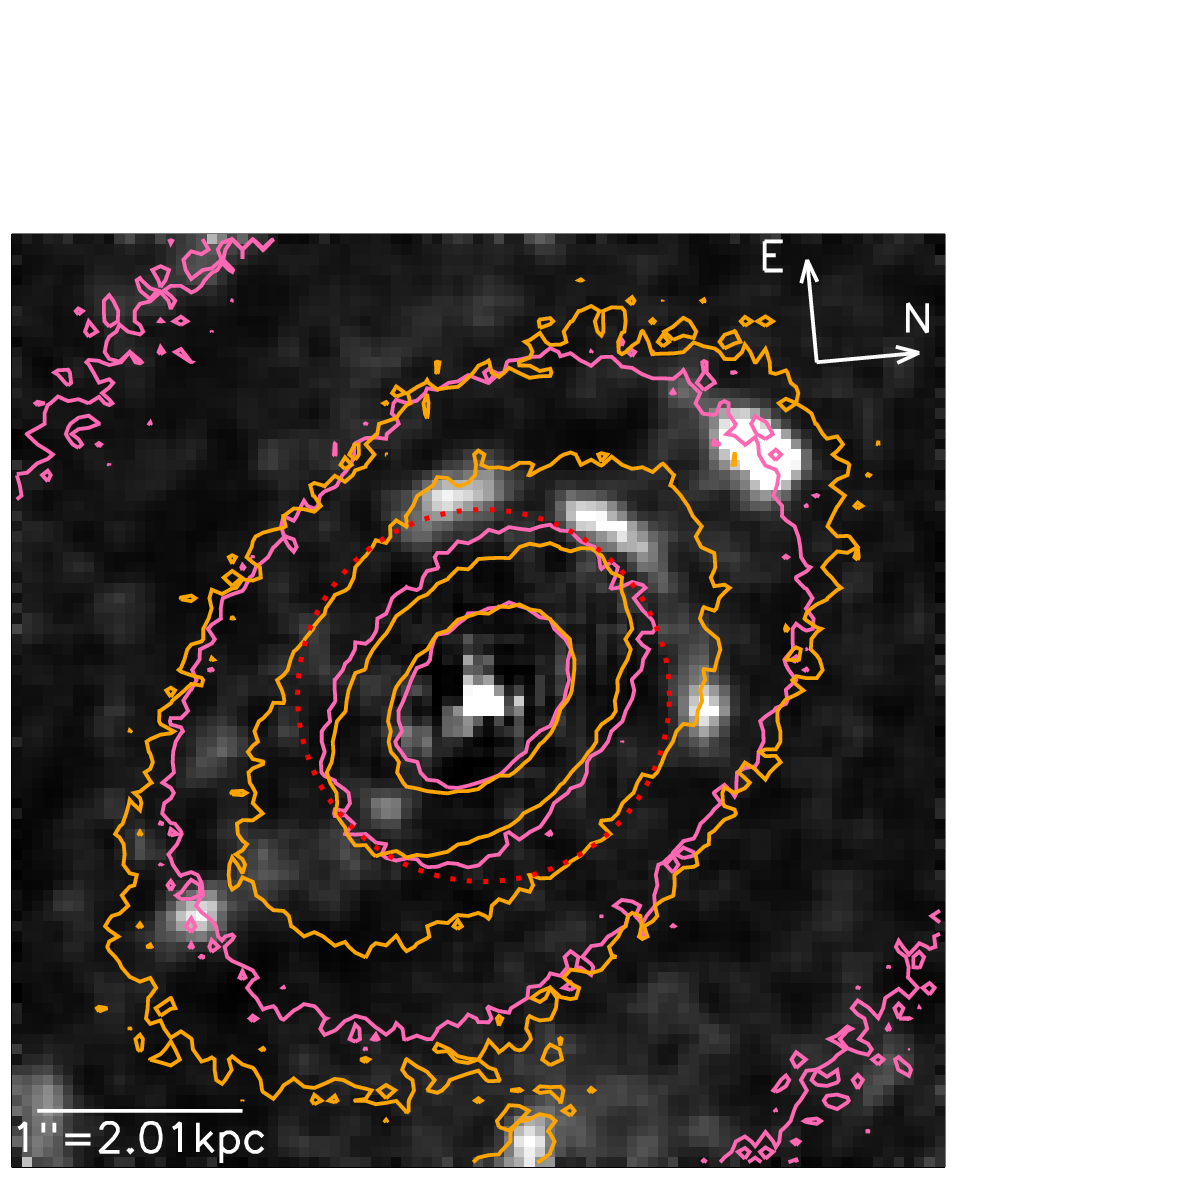
\includegraphics[width=.9\linewidth]{fig/paper_lensmass_brightness_compare.ps}
  \caption{Comparison of mass and light.}
  \label{fig:lenscompareboth}
\end{subfigure}
\caption{Comparison of the observed F814W/I-band surface brightness distribution (Panel (a) and orange contours) and predicted mass distribution from lensing constraints (Panel (b) and pink contours). To allow for a qualitative comparison of the contours in Panel (c), the light distribution was turned into a mass distribution by multiplication with the total mass-to-light ratio inside the Einstein radius $\Upsilon_\text{I,tot}^\text{ein}$ in Table \ref{tab:einsteinML}. The Einstein radius is overplotted as red dotted circle. The uncertainties in the mass model in the second column of Table \ref{tab:bestfitlensmodel} were translated into random Monte Carlo noise in the mass contours. The smooth black contours correspond to the best fit model in the first column of Table \ref{tab:bestfitlensmodel}. The background in Panel (c) shows again the surface brightness subtracted center of the galaxy to make the lensing images visible.}
\label{fig:lenslightcompareALL}
\end{figure*}

\subsection{JAM based on surface brightness} \label{sec:results_JAM_SB}

\paragraph{JAM with lens mass model.} Our first JAM model uses the mass distribution which we found from lensing constraints in Section \ref{sec:results_lensing} to generate an independent prediction for the $v_\text{rms}$ curve following the procedure in Section \ref{sec:model_JAM}. In addition to the flat rotation curve model with $\alpha = 1$ in Table \ref{tab:bestfitlensmodel}, we also investigate a lens model, which was found as a best fit to the lensing images when assuming a slightly rising rotation curve slope of $\alpha=1.1$. The predictions are compared with the data in Figure \ref{fig:JAM_modelL}. The agreement between the lensing prediction and the observed kinematics within $R' \sim 3$ arcsec is striking, especially around the Einstein radius. The $\alpha = 1$ model fits the wings nicely, while the $\alpha = 1.1$ model recreates almost exactly the observed central dip. The sharp drop in $v_\text{rms}$ around $R' \sim 3$ arcsec cannot be reproduced, however. But outside of the Einstein radius our lensing models are only extrapolations and the true constraint is around the Einstein radius.

%==================================================================

\begin{figure}
  \centering
  \includegraphics[height=6cm]{fig/lensing_JAM_comparision.ps}
  \caption{Comparison (not a fit!) of the symmetrized stellar $v_\text{rms}$ data of J1331 (blue dots) with JAM models generated from mass distributions which were independently derived from lensing constraints in Section \ref{sec:results_lensing}. The red solid line corresponds to the lens model for a flat rotation curve ($\alpha = 1$) in Table \ref{tab:bestfitlensmodel}; the green line is a best fit lens model found analogously from the image positions, but for a fixed rotation curve slope of $\alpha = 1.1$. For the JAM modelling a best fit MGE to the lens mass models were used, as well as the observed surface brightness MGE in Table \ref{tab:MGEF814W}, assuming velocity isotropy $\beta_z = 0$ and an inclination of $i = 70^\circ$.The red and black dotted lines are the Einstein radius and the effective half-light radius, respectively.}
  \label{fig:JAM_modelL}
\end{figure}

%==================================================================


\paragraph{JAM with "mass-follows-light" and velocity anisotropy.} Our second JAM model is a mass-follows-light model, which are often used in dynamical JAM modelling (e.g. \citet{GlennEC,Cap06}), where the mass distribution ins generated by multiplying the intrinsic light distribution $\nu(R,z)$ (the MGE given in Table \ref{tab:MGEF814W} deprojected according to the inclination) by a constant total mass-to-light ratio  $\Upsilon_\text{I,tot}^\text{dyn}$. This assumes that the dark matter is always a constant fraction of the total matter distribution everywhere. This simplified model sometimes gives good representations of the inner parts of galaxies, where the stellar component dominates. Testing this model for J1331 is also motivated by our findings from lensing in Section \ref{sec:results_lensing}, where around the Einstein radius total and luminous mass seem to have a similar distribution.
\\In addition to the free fit parameter  $\Upsilon_\text{I,tot}^\text{dyn}$, we also allow for a overall constant but non-zero velocity anisotropy $\beta_z$. The best fit is found by minimizing $\chi^2$ between the $v_\text{rms}$ data and model prediction and is demonstrated in Figure \ref{fig:JAM_modelA2}. For $\beta_z$ we impose the fitting limits $\beta_z \in [-0.5,+0.5]$. While the outer parts of galaxies often show radially biased velocity anisotropy up to $\sim 0.5$ (from dynamical modelling of observed elliptical galaxies (e.g. \citet{Kronawitter2000}) and cosmological simulations (e.g. \citet{2004MNRAS.352..535D,2001ApJ...557..533F}), the centers of galaxies are near-isotropic or have  negative velocity anisotropy \citep{2003ApJ...583...92G}. Only in extreme models (e.g. around in-spiralling supermassive black holes \citep{1997NewA....2..533Q}) velocity anisotropies as low as $\sim -1$ have been found. A lower limit of $\beta_z \geq -0.5$ is a realistic assumption for J1331, for which we do not expect extreme dynamical conditions. The best fit in Figure \ref{fig:JAM_modelA2} however strives to very negative velocity anisotropies to be able to get the deep central dip in the  $v_\text{rms}$ curve. But $\beta_z = -0.5$ is not even a remotely agreeable fit and lower anisotropies are not to be expected and realistic. We also tested radial profiles for $\beta_z(R)$ of the form proposed by \citet{BaesVanHese}, which was however equally unable to reproduce the data. We conclude, that this is due to the well-known degeneracy between anisotropy and mass profile [TO DO: REF] and the mass-follows-light model is \emph{not} a good representation of the mass distribution in J1331's inner regions.


%==================================================================

\begin{figure}
  \centering
  \includegraphics[height=6cm]{fig/jam_A2_vrms.ps}
  \caption{Comparison of the symmetrized $v_\text{rms}$ data of J1331 (blue dots) with a best fit dynamical JAM model (solid red line) assuming mass-follows-light and with two free parameters: $\Upsilon_\text{I,tot}^\text{dyn}$, the total I-band mass-to-light ratio found from dynamics, which converts the observed surface brightness in Table \ref{tab:MGEF814W} into a mass distribution, and the velocity anisotropy parameter $\beta_z$. The ``best'' fit is $\Upsilon_\text{I,tot}^\text{dyn} = 4.8 \pm 0.1$ and $\beta_z = -0.5$, where the latter is however pegged at the lower limit of the allowed value range. This is obviously not a good model.}
  \label{fig:JAM_modelA2}
\end{figure}

%==================================================================

\paragraph{JAM with increasing mass-to-light ratio.} In Section \ref{sec:results_lensing} we found from the lensing, that the light distribution might drop faster with radius than the mass distribution. This would correspond to a radially increasing total mass-to-light ratio. As velocity anisotropy alone cannot explain the observed kinematics in a simple a mass-follows-light model, we now allow for an mass-to-light ratio gradient in the JAM modelling to generate a mass model from the light distribution in Table \ref{tab:MGEF814W}. We do this by assigning each of the five Gaussians in the MGE its own total mass-to-light ratio $\Upsilon_{\text{I,tot,}i}$ and replace the total luminosity in Equation \ref{eq:centralItotalL} $L_i$ with the Gaussians total Mass $M_i = \Upsilon_{\text{I,tot,}i} L_i$. We treat the five $\Upsilon_{\text{I,tot,}i}$ as free parameters and only require that $\Upsilon_{\text{I,tot,}j} \geq \Upsilon_{\text{I,tot,}i}$ when the corresponding $\sigma_j \geq \sigma_i$ to ensure an overall mass-to-light ratio that is increasing with radius.
\\Figure \ref{fig:enclMass_modelG} shows the (local projected) mass-to-light ratio gradient generated by the best fit to the dynamics data, which rises from $\Upsilon_\text{I,tot} = 2.53$ in the center and approaches a value of $\Upsilon_\text{I,tot}$ outside of the fitted region at $R'\gtrsim 3$ arcsec of $\Upsilon_\text{tot} = 7.60)$. The central mass-to-light ratio corresponds to the mass-to-light ratio found in Table \ref{tab:previousresults} based on the results of \citet{SWELLSI} assuming a stellar population with an \citet{Chabrier2003} initial mass-function (IMF, see also Section \ref{sec:MLdiscussion}), $\Upsilon_\text{I,*}^\text{chab} = 2.5 \pm 0.6$. When assuming that galaxy bulges are generally older and redder in the center [TO DO: REF], i.e. $\Upsilon_\text{I,*}$ is rather dropping with increasing radius than increasing, the strong rise of $\Upsilon_\text{I,tot}(R')$ might be due to a strong contribution of dark matter in J1331.
\\Figure \ref{fig:JAM_modelG} shows that the best fit model greatly reproduces the central dip in the $v_\text{rms}$ curve, even though it has slight problems fitting the drop around $R' \sim 4$ arcsec. The latter might be because we only allowed the $\Upsilon_\text{I,tot}(R')$ to rise. A slight drop could be expected when the reddish bulge turns into the bluish disk and the contribution of the stellar component becomes less due to a lower $\Upsilon_\text{I,*}$ for younger and bluer populations.
\\In Figure \ref{fig:enclMass_modelG} we overplot the enclosed mass profile with the Einstein mass $M_\text{ein} = (7.77 \pm 0.33) \cdot 10^{10} M_\odot$ at the Einstein radius found from lensing in Table \ref{tab:bestfitlensmodel}. The agreement between the Einstein mass and the independently found $M(<R_\text{ein}) = 7.49 \cdot 10^{10} M_\odot$ from dynamical modelling is striking.


%==================================================================

\begin{figure*}
\centering
\begin{subfigure}{.5\textwidth}
  \centering
  \includegraphics[height=6cm]{fig/jam_G_vrms.ps}
  \caption{Comparison of $v_\text{rms}$ data and best fit model.}
  \label{fig:JAM_modelG}
\end{subfigure}%
\begin{subfigure}{.5\textwidth}
  \centering
  \includegraphics[height=6cm]{fig/jam_G_enclMass.ps}
  \caption{Projected local mass-to-light ratio profile and enclosed mass.}
  \label{fig:enclMass_modelG}
\end{subfigure}
\caption{JAM model found by fitting an increasing total mass-to-light ratio $\Upsilon_\text{I,tot}(R')$ profile used to generate a mass model from the light distribution.  This is done by assigning a different mass-to-light ratio to each Gaussian in the MGE in Table \ref{tab:MGEF814W}. \emph{Panel (a):} Comparison between the stellar $v_\text{rms}$ data (blue points) and the best fit model (green line). \emph{Panel (b):} Enclosed mass inside the projected radius $R'$ on the sky (green line, right axis) and projected mass-to-light profile $\Upsilon_\text{I,tot}(R')$ along the major axis (blue line, left axis) of the best fit model. The enclosed mass curve is overplotted with the independent finding for the Einstein mass $\pm 4 \%$ in Table \ref{tab:bestfitlensmodel} (red dot) at the Einstein radius (red dotted line). The best fit mass-to-light ratios of the first four Gaussians are plotted against each Gaussians $\sigma$ (yellow stars). The two Gaussians with the largest $\sigma$ (the fifth is not shown) have the same best fit mass-to-light ratio. Overplotted is also the effective half-light ratio $R_\text{eff}$ (black dotted line).}
\label{fig:modelG}
\end{figure*}

%==================================================================
\subsection{JAM with a NFW Dark Matter Halo} \label{sec:results_JAM_NFW}

\paragraph{Including a NFW halo.} The dynamical modelling attempts in the previous sections suggest that J1331's inner regions have a slightly more roundish and at large radii more massive mass distribution than expected from the distribution of stars alone. A dark matter halo in addition to the stellar component could explain these findings. We therefore proceed by modelling the mass distribution with a) a stellar component, which we get from the light MGE in Table \ref{tab:MGEF814W} times a constant stellar mass-to-light ratio $\Upsilon_*$), and b) a spherical NFW dark matter component \citep{Navarro+1995c,NFW96}. In the JAM modelling we use a 10-Gaussian MGE fit to the classical NFW profile
\begin{equation*}
\rho_\text{NFW}(r) \propto 1 / \frac{r}{R_\text{s,NFW}} \left( 1 + \frac{r}{R_\text{s,NFW}} \right)^2.
\end{equation*}
The NFW halo has two free parameters, the scale length $R_\text{s,NFW}$ and a parameter describing the total mass of the halo. We use $v_\text{200}$, which is the circular velocity at the radius $r_\text{200}$ within which the mean density of the halo is 200 times the cosmological [TO DO: how to express this] critical density, i.e.
\begin{eqnarray*}
M_\text{200} &=& M(<r_{200})\\
\frac{M_{200}}{ \frac 43 \pi r_{200}^3} &=& 200 \rho_\text{crit}(z=0) \\
v_\text{200} &=& \sqrt{\frac{GM_{200}}{r_\text{200}}}
\end{eqnarray*}
with $\rho_\text{crit}(z=0)=1.43 \cdot 10^{-7} M_\odot / \text{pc}^3$ in the WMAP5 cosmology by \citet{WMAP5cosm}. How much the mass is concentrated in the center of the NFW halo is given by the concentration of the NFW halo defined by $c_{200}\equiv r_{200} / R_{s,NFW}$. [TO DO: so toll ist das mit der Radiusbenennung noch nicht.????]. There is a close relation between the concentration and halo mass in simulations \citep{NFW96}. \citet{Maccio08} found this relation for the WMAP5 cosmology \citep{WMAP5cosm} to be
\begin{equation}
\langle \log c_{200} \rangle (M_{200}) = 0.830 - 0.098 \log \left(h \frac{M_{200}}{10^{12} M_\odot} \right) \label{eq:Maccio08}
\end{equation}
(their equation 10), with a Gaussian scatter of $\sigma_{\log c_{200}} = 0.105$ (their table A2).


\paragraph{Modelling.} The full set of fit parameters is $(\Upsilon_{I,*},R_\text{S,NFW},v_{200},\beta)$ [TO DO: $\beta$ or $\beta_0$???] [TO DO: Einheitlich $\Upsilon_{I,*}$????], where $\beta$ is the constant velocity anisotropy parameter (see \S\ref{sec:model_JAM}). We will investigate this parameter space with a MCMC \citep{emcee} and use priors for the halo parameters to guide the fit to a realistic NFW halo shape.
\\\citet{Dutton10} give a relation for halo vs. stellar mass for late-type galaxies. For an Chabrier IMF stellar population they found
\begin{equation*}
y = y_0 \left( \frac{x}{x_0} \right)^\alpha \left[ \frac 12 + \frac 12 \left(\frac{x}{x_0} \right)^\gamma \right]^{(\beta - \alpha)/\gamma},
\end{equation*}
where $x= m_*$ [$M_\odot h^{-2}$] is the stellar mass, $y = \frac{\langle M_{200}\rangle}{m_*}$ and $\langle M_{200}\rangle$ [$M_\odot h^{-2}$] is the mean halo mass. The parameters for the mean and $2\sigma$ error curves for this relation are$\alpha = -0.5\pm0.15$, $\beta = 0$, $\gamma = 1.0$, $\log_{10} x_0 = 10.4$, $\log_{10} {y_0}_{-0.24}^{+0.28}$ \citet{Dutton10}. Using the stellar mass estimate for J1331 from \citet{SWELLSI} $m_* = (1.06 \pm 0.25) \cdot 10^{11} M_\odot$ for the Chabrier IMF estimate [TO DO: introduce somewhere], we find ${v_{200}} = (202_{-33}^{+44})_{-13}^{+12}$. The first of the two quoted errors is due to the $2\sigma$ scatter in the relation by \citet{Dutton10}. The second error is the propagated error due to the uncertainty in the stellar mass. We use this as a rough estimate for the halo of J1331 and as Gaussian prior on $v_{200}$, 
\begin{equation*}
p(v_{200}) = \mathscr{N}(200 \text{km/s} ,40 \text{km/s}).
\end{equation*}
\\We also use the concentration vs. halo mass relation by \citet{Maccio08} in Eq. (\ref{eq:Maccio08}) as a prior on the concentration, i.e.
\begin{equation*}
p(\log c_{200} \mid v_{200}) = \mathscr{N}\left(\langle \log c_{200} \rangle (M_{200}) \mid 0.105 \right).
\end{equation*}
\\For the velocity anisotropy parameter $\beta$ we will again employ a uniform prior 
\begin{equation*}
p(\beta) = \mathscr{U}(-0.5,+0.5)
\end{equation*}
to exclude very unrealistic anisotropies. The full prior used is then
\begin{equation*}
p(\Upsilon_{I,*},R_\text{S,NFW},v_{200},\beta) = \frac{1}{\ln\left( 10 R_{s,NFW}\right)} p(\log c_{200} \mid v_{200}) \cdot p(v_{200}) \cdot p(\beta), 
\end{equation*}
where the factor $1/\ln\left( 10 R_{s,NFW}\right)$ is the Jacobian of the transformation from the halo parameters $(v_{200},\log c_{200})$ [TO DO: introduce concentration] to $(v_{200},R_{s,NFW})$.
\\We restrict the $v_\text{rms}$ fit to a region $R' \lesssim 3.5$ arcsec, approximately within the effective half-light radius $R_\text{eff} = 2.6$ arcsec  [TO DO: make sure R' everywhere ???]. We also include the Einstein mass $M(<R_\text{ein}$ with a 10\% error as an additional constraint in the fit. 


\paragraph{Result.} Figure \ref{fig:modelB4_triangle} shows the posterior probability distribution of the fit sampled with an MCMC. Overplotted are also the priors used to constrain the NFW halo. The best fit parameters are summarized in Table \ref{tab:modelB4_bestfit}. We find that the best fit NFW halo strives to be more massive and with a higher concentration than  proposed by the prior. At the same time the model prefers again very negative velocity anisotropies; the sample with the highest probability is pegged at the lower limit of the prior. Both, the concentrated halo and the low anisotropy are needed to reproduce the central dip of the $v_\text{rms}$ curve. [TO DO: Rewrite. Not very good.]

The first panel in Figure \ref{fig:modelB4_vrot} shows the mean best fit values from Table \ref{tab:modelB4_bestfit}.

We also fitted a model with a cored logarithmic dark matter halo. The cored halo models are in general slightly less massive than the NFW halo and therefore fitt the outer regions of J1331 better. However, the density profile of the cored halo as well as the I-band light distribution within the plane drop as $\rho(r) \propto r^{-2}$, there is a strong degeneracy between the stellar mass and the dark matter. Overall we were not able to give tight constraints on the cored logarithmic halo.

\begin{figure*}
\centering
\includegraphics[width=0.9\linewidth]{fig/B4_contour_plot_short.ps}
\caption{Posterior probability distribution sampled with MCMC (red dots and histograms) for a JAM model with NFW halo, parametrized by $R_\text{s,NFW}$ and $v_\text{200}$, a stellar mass distribution generated from the I-band MGE in Table \ref{tab:MGEF814W} and a constant stellar mass-to-light ratio $\Upsilon_{I,*}$, and constant velocity anisotropy $\beta_z$. Shown are also the priors used for J1331's NFW halo, $\mathscr{N}(200 \text{km/s},40 \text{km/s})$ (green) and the concentration vs. halo mass relation by \citet{Maccio08} from Eq. (\ref{eq:Maccio08}) in terms of $v_{200}$ vs. $R_\text{s,NFW}$ with $1\sigma$ scatter (blue). The MCMC samples are color coded according to their probability (darker red for higher probability); the sample point with the highest probability is marked by a black diamond. The black cross is the mean of the distribution and the ellipses are derived from the covariance of matrix of the sample set and correspond approximately to $1\sigma$ (black solid ellipse) and $2\sigma$ (black dotted ellipse). The histograms of the marginalized 1D distributions are overplotted by the mean (black solid lines) and $1\sigma$ error (black dashed lines), whose values are also quoted in the figure and in Table \ref{tab:modelB4_bestfit}. The grey diamonds mark a random sub-selection of 12 samples; the corresponding models are shown in Figure \ref{fig:modelB4_models}.}
\label{fig:modelB4_triangle}
\end{figure*}

\begin{table*}
\centering
\begin{tabular}{llrcl}
\hline
stellar I-band mass-to-light ratio & $\Upsilon_{I,*}$ & 4.2 & $\pm$ & 0.2\\
velocity anisotropy & $\beta_z$ & -0.4 & $\pm$ & 0.1 \\
NFW halo scale length & $R_\text{s,NFW}$ [kpc] & 40 & $\pm$ & 20\\
NFW halo virial velocity & $v_{200}$ [km/s] & 240 & $\pm$ & 40\\
NFW halo concentration & $c_{200}$ & 8 & $\pm$ & 2 \\
NFW halo mass & $M_{200}$ [$10^{12} M_\odot$] & 5 & $\pm$ & 2\\
\hline
\end{tabular}
\caption{Summary of the best fit parameters of the JAM model with NFW halo from the MCMC exploration in Figure \ref{fig:modelB4_triangle}. The halo mass and concentration are calculated from the the best fit $R_\text{s,NFW}$ and $v_{200}$.}
\label{tab:modelB4_bestfit}
\end{table*}

\begin{figure*}
\centering
\begin{subfigure}{\textwidth}
  \centering
  \includegraphics[width=0.8\linewidth]{fig/B4_rms_error_curves.ps}
  \caption{Comparison of the $v_\text{rms}$ data with the best fit JAM models.}
  \label{fig:modelB4_vrms}
\end{subfigure}
\begin{subfigure}{.48\textwidth}
  \centering
  \includegraphics[width=0.9\linewidth]{fig/B4_jam_profiles_errors_short_vcirc.ps}
  \caption{Circular velocity curve.}
  \label{fig:modelB4_vcirc}
\end{subfigure}%
\hspace{.02\textwidth}
\begin{subfigure}{.48\textwidth}
  \centering
  \includegraphics[width=0.9\linewidth]{fig/B4_jam_profiles_errors_short_projmass.ps}
  \caption{Enclosed mass profile.}
  \label{fig:modelB4_enclMass}
\end{subfigure}
\caption{Best fit JAM model including a NFW halo and velocity anisotropy with parameters given in Table \ref{tab:modelB4_bestfit}. The 12 lines shown correspond to the 12 models randomly drawn from the posterior probability distribution and marked as grey diamonds in Figure \ref{fig:modelB4_triangle}. Overplotted are the Einstein radius (red dotted line) and the effective half-light radius (black dotted line). The blue dashed line marks the radius within which the data and model were fitted. \emph{Panel a)} shows the comparison of the symmetrized $v_\text{rms}$ data (solid blue points) with the best fit JAM models including a NFW halo (red solid lines). Also shown is the non-symmetrized data at larger radii (open blue dots) and an extrapolation of the best fit models, using the same model parameters but the I-band surface brightness MGE for the outer regions of J1331 derived from the Ellipse model (red dashed lines). \emph{Panel b)} shows the circular velocity curve of the total mass (green), and separately the contribution of the stellar mass (yellow, again generated from the MGE in Table \ref{tab:F814WMGE}) and dark matter (grey). \emph{Panel c)} shows the corresponding enclosed mass profile. Overplotted is also the Einstein mass at the Einstein radius with a 10\% error, which was used in the fit as an additional constraint.[TO DO: radius benennungen sind irgendwie verrutscht]}
\label{fig:modelB4_models}
\end{figure*}



\paragraph{Rotation curve.} Following the procedure in \S\ref{sec:model_JAM} we find the rotation curve from the best fit mean model in Table \ref{tab:modelB4_bestfit} by fitting the rotation parameter $\kappa'$ to the symmetrized $v_\text{rot}$ data within $R' = 3.5$ arcsec. The best fit with $\kappa' = 0.76$ is shown in the second panel of Figure \ref{fig:modelB4_vrot}. The third panel gives the dispersion that was calculated simply by $\sigma = \sqrt{v_\text{rms}^2 - v_\text{rot}^2}$. Our assumptions for $\kappa(R)$ nicely reproduce a $v_\text{rot}$ model with counter-rotating core. Although we fitted $v_\text{rot}$ only to the inner regions, the extrapolation to large radii fits the data also very well. While the dispersion $\sigma$ in the center fits by construction quite good, there is a huge discrepancy at large radii. The predicted dispersion is much larger than the data; we would expect the disk rotationally supported and therefore have a low velocity dispersion; especially dispersions as high as $\sim 200 km/s$ are more likely to be observed in the pressure supported bulges of galaxies. There \emph{might} be something unexpeted with the $\sigma$ measurements around $\sim 5$ arcsec, but at large radii the the best fit model NFW halo is simply too massive. 

\begin{figure*}
\centering
\includegraphics[width=0.7\linewidth]{fig/B4_rms_rot_curves_best_model.ps}
\caption{Generating the rotation curve from the JAM model with NFW halo and constant velocity anisotropy with the mean parameters in Table \ref{tab:modelB4_bestfit} and with the best fit rotation parameter $\kappa' = 0.76$ in Eq. (\ref{eq:kappa_profile}) (red solid lines). The second velocity moment in the first panel and the first velocity moment in the second panel with the additional fit parameter $\kappa'$ were fitted to the symmetrized data (solid blue points). The velocity dispersion is simply $\sigma = \sqrt{v_\text{rms}^2 - v_\text{rot}^2}$. At larger radii we compare the unsymmetrized data (open blue dots), the gas kinematics from \citet{SWELLSV} (green diamonds) and a JAM model using the same model parameters but the light distribution MGE generated from the Ellipse model in Figure [TO DO: REF FIGURE] as a prediction for the outer regions of J1331 (red dashed lines). The central regions are very well reproduced and we can also greatly predict the rotation curve at larger radii. Only at larger radii the $v_\text{rms}$ and $v_\text{rot}$ overestimate the measurements, probably due to a too massive NFW halo.}
\label{fig:modelB4_vrot}
\end{figure*}

%------------------------

%------------------------
\section{Discussion and Conclusion} \label{sec:Discussion}
We've presented different dynamical models of the central region of J1331, some of them capturing the observed kinematics well, but none of them work both at small and large radii. In the following we will discuss possible reasons for these deviations by also comparing our results to previous work.

\subsection{On J1331's Stellar Mass-to-Light Ratio} \label{sec:MLdiscussion}

Further knowledge of the stellar populations within J1331 and their initial mass functions (IMF) would be useful. In particular a sophisticated guess for the \emph{stellar} mass-to-light ratio in J1331's bulge could be compared to our very reliable measurement of the \emph{total} mass-to-light ratio inside the Einstein radius (see Table \ref{tab:einsteinML} ) to support or contradict the presence of a lot of dark matter in the bulge. \\

Traditional choices for the IMF are the bottom-heavy IMF by \citet{Salpeter1955},
$$\xi(m) \propto m^{-x}, x=2.35,$$
(where $\xi(m) \diff m$ is the number of stars with mass $m$ in $[m,m+\diff m]$) and the IMFs by \citet{2002Sci...295...82K} and \citet{Chabrier2003}, which are in agreement with each other and predict less low-mass stars. \\

\citet{Ferreras} found a relation between the central stellar velocity dispersion $\sigma_0$ in early-type galaxies and the IMF slope. A higher $\sigma_0$ suggests a more bottom-heavy IMF. For an unimodal (Salpeter-like) IMF and a $\sigma_0 \propto 200 $ km/s for J1331 (see Figure \ref{fig:kinematics}) they predict $x \approx 2.33$ (see Figure 4 in \citet{Ferreras}), which is close to the standard Salpeter slope. These findings are supported by \citet{2014MNRAS.438.1483S}, who found for SDSS galaxies also a relation between unimodal (single power-law) IMF slope and stellar velocity dispersion. Their Table 2 lists $x(\sigma_*=190 \pm 20 \text{ km s}^{-1}) = 2.08 \pm 2.08$ and $x(\sigma_*= 230 \pm 20 \text{ km s}^{-1}) = 2.33 \pm 0.4$. When assuming a bi-modal (Kroupa-equivalent-like) IMF, \citet{Ferreras} predict $x \approx 2.85$ (see Figure 4 in \citet{Ferreras}) for J1331's central velocity dispersion. This is more bottom-heavy than the standard \citet{2002Sci...295...82K} IMF. Overall the central velocity dispersion suggests a rather bottom-heavy IMF J1331's bulge and therefore large stellar mass-to-light ratio.\\

\citet{SWELLSI} estimated J1331's stellar bulge mass given a Salpeter IMF and measured the I-band AB magnitude of the bulge. Transformed to a stellar I-band mass-to-light ratio (see Table \ref{tab:previousresults}) this would correspond to $\Upsilon_\text{I,*}^\text{Salpeter} = 4.7 \pm 1.2$.\\

We compare our findings of the stellar mass-to-light ratios with the study by \cite{SWELLSV}: \cite{SWELLSV} found that the bulge of J1331 has an IMF more bottom-heavy than the Salpeter IMF from fitting a NFW halo to (1) the Einstein mass and (2) gas kinematics at larger radii $\gtrsim 8$ arcsec. In Section \ref{sec:results_JAM_NFW} we fitted the stellar kinematics within $\sim 3.5$ arcsec and the Einstein mass with a NFW halo and the best fit $\Upsilon_\text{I,*}^\text{dyn} = 4.2 \pm 0.2$ (see Table \ref{tab:modelB4_bestfit}) indicates a less bottom-heavy IMF than the Salpeter IMF. \cite{SWELLSV}  found systematically lower NFW halos ($v_\text{circ}(5\text{arcsec}) \sim 120 \text{km s}^{-1}$ according to their Figure 2) than we did ($v_\text{circ}(5\text{arcsec}) \sim 200 \text{km s}^{-1}$, see Figure \ref{fig:kinematics}). We note however, that our results would be much closer to those by \citet{SWELLSV}, if we only used the lensing results at small radii as they did: The total mass-to-light ratio of $\Upsilon_\text{I,tot}^\text{ein} = 5.6$ inside the Einstein radius (see Table \ref{tab:einsteinML}). In case of a lower mass dark matter halo, the largest contribution to this mass-to-light ratio would then be stellar mass. And the corresponding IMF would be more bottom-heavy than Salpeter,  like what \citet{SWELLSV} found. The circular velocity curve $v_\text{circ}(R) = \left. sqrt{R \frac{\partial \Phi}{\partial R}} \right|_{z=0}$ \citet{SWELLSV} find for J1331 peaks at $v_\text{circ}(R\sim0.9 \text{arcsec}) \sim 350 \text{km s}^{-1}$ (from lensing constraints only) and at $v_\text{circ}(R\sim0.9 \text{arcsec}) \sim 370 \text{km s}^{-1}$ (when including a dark matter halo and gas kinematics in the fit). We get a very similar circular velocity curve (at least at small radii) for a mass-follows-light model with constant $\Upsilon_\text{I,tot}^\text{ein} = 5.6$, which peaks at $v_\text{circ}(R\sim0.9 \text{arcsec}) \sim 360 \text{km s}^{-1}$. From this comparison follows, that the model by \citet{SWELLS} corresponds approximately to a mass-follows-light model in the inner regions of J1331. In Section \ref{sec:results_JAM_SB} however we showed, that this is \emph{not} a good model for J1331 and won't be able to reproduce the central stellar $v_\text{rms}$ dip. On the other hand, because our NFW JAM models fail to predict the stellar kinematics at large radii, the true halo parameters are more likely closer to the findings by \citet{SWELLSV}.\\

All of this leaves the central dip unexplained: It cannot be due to tangential velocity anisotropy in the center alone (see Section \ref{sec:results_JAM_SB}, Figure \ref{fig:JAM_modelA2}). It also cannot be explained by a strong contribution of dark matter inside the bulge together with a moderate tagential velocity anisotropy, because the corresponding dark matter halos would still be too massive to fit the data in the outer regions (see Section \ref{sec:results_JAM_NFW}, Figure \ref{fig:modelB4_vrms}]).\\

An alternative JAM model was introduced in Section \ref{sec:results_JAM_SB}, where we used the surface brightness distribution without a halo component but together with an increasing mass-to-light ratio. We found that such a model would be perfectly consistent with the lensing results and predict a total mass-to-light ratio in the center of J1331 of  $\Upsilon_\text{I,tot}(R\sim0) = 2.53$. This is very close to the stellar mass-to-light ratio we got from \citet{SWELLSI} estimates of the bulge's stellar mass using the Chabrier IMF $\Upsilon_\text{I,*}^\text{Chabrier} = 2.5 \pm 0.6$, i.e. less bottom-heavy (more bluish) population.\\

Another feature in the stellar kinematics, that none of our JAM models was able to reproduce in the slightest and which we therefore excluded in the modelling, was the dip in $v_\text{rms}$ around $\sim 6$ arcsec, which occurs around the transition from bulge to disk (see Figure [TO DO: 1b]).\\

The above discussion motivates the following speculation: In the absence of a strong dark matter contribution in the center, the overall stellar-mass-to-light ratio within the Einstein radius indicates a bottom-heavy IMF close to the Salpeter IMF, consistent with estimates from the velocity dispersion. At the same time the central dip can then be only explained, if there was an increase in stellar mass-to-light ratio with radius \textit{within} the bulge. \emph{If} there was a central stellar population with an IMF close to the \citet{Chabrier2003} IMF, surrounded by a more bottom-heavy population, the central stellar kinematics would be well explained and be fully consistent with the lensing results. (According to Figure \ref{fig:lenscompareboth} the lensing result might not predict a mass to light ratio gradient inside $R_\text{ein}$, but then again the mass slope $alpha=1$ was only weakly constrained.) The disk of J1331 has a lower $\Upsilon_\text{I,*}$ than the bulge (see Table \ref{tab:previousresults} according to \citet{SWELLSI}). Such a drop in $\Upsilon_\text{I,*}$ at the transition region from bulge to disk around $\sim 5$ arcsec could lead to the observed drop in $v_\text{rms}$, while an increasing contribution of a lower mass dark matter halo at larger radii as found by \citet{SWELLSV}, would recover the kinematics in the out regions of J1331's disk.\\



[TO DO: Rewrite the paper such, that it's main message is, that there is a strong indication of increasing stellar mass-to-light ratio in the center of the galaxy, i.e. a bluish core, because neither velocity anisotropy, neither a strong dark matter contribution alone can explain all dynamical signatures. "Evidence from Lensing and Dynamics for a bluish core in the center of J1331" as a possible alternative title??? Eher nicht...]

[TO DO: Einheitlich: $Upsilon_{I,*}^{comment}$, $\Upsilon_\text{I,tot}^\text{ein}$]

\begin{table*}
\centering
\begin{tabular}{cccccc}
\hline\hline
& & \multicolumn{2}{c}{Chabrier IMF} & \multicolumn{2}{c}{Salpeter IMF}\\
      &  $L$ [$10^{10}L_{\odot}$]                & $M_*$ [$10^{10}M_\odot$]               & $\Upsilon_\text{I,*}^\text{chab}$ & $M_*$ [$10^{10}M_\odot$] & $\Upsilon_\text{I,*}^\text{Salpeter}$ \\\hline
bulge &   $3.10 \pm 0.15 $  & $7.8 \pm 1.8$ & $2.5 \pm 0.6$ & $14.5 \pm 3.7 $ & $4.7 \pm 1.2$ \\
disk  &   $2.35 \pm 0.11 $  & $2.9 \pm 0.7$ & $1.2 \pm 0.3$ & $5.2 \pm 1.1$ & $2.2 \pm 0.5$ \\
total &   $5.45 \pm 0.19$ & $10.6 \pm 1.9$& & $19.7 \pm 3.9$&\\\hline
\end{tabular}
\caption{Total I-band luminosity, stellar mass and mass-to-light ratio, calculated from the I-band AB magnitudes and stellar masses found for J133's bulge and disk by \citet{SWELLS} (their table 2) for comparison with this work. The transformation from AB magnitudes to the Johnson-Cousins I-Band used the relation $I[\text{mag}] = I[\text{ABmag}] - 0.309$ from \citet{FG1994} (their table 2). For the conversion from apparent magnitude to total luminosity the redshift $z=0.113$ \citet{SWELLSIII} was turned into a luminosity distance using the cosmology by \ref{WMAP5cosm}. }
\label{tab:previousresults}
\end{table*}
\subsection{Does J1331 have a Merger History?}

\paragraph{TO DO: Stuff to mention}
\begin{itemize}
\item J1331 has a counter-rotating stellar component.
\item suggests that there was a process where two components with angular momenta oriented in opposite directions were involved
\item 1. scenario: accretion of gas on retrograde orbits and subsequent star formation
\item --> counter-rotating component is younger than the rest of the galaxy
\item argument against: To form enough stars such taht the net rotation of the large and massive core is retrograde, a very large amount of gas would have had to be accreted - which is not very likeliy [TO DO" REF: KLEINEBERG 2011] 
\item 2. scenarios: Major mergers of similarly massive galaxies
\item argument against: major merger products are often quiescent, elliptical galaxies [TO DO: REF: TOOMRE TOOMRE 1972]
\item 3. sencaro: minor merger
\item --> dissipationless accretion of a satellite on retrograde orbit [TO DO: REF: KORMENDY 1984] with dense core to survive and spiral to core due to tidal friction
\item --> counter-rotating component would be younger, as star formation in low-mass satellite galaxies occurs later [TO DO: REF]
\item if the counter-rotating component is younger needs to be tested by detailed stellar population analysis
\item Minor merger effects in elliptical galaxies have been studied e.g. by [TO DO:REF: BALCELLS AND QUINN 1990]
\item large bulges of sporals or ellipticals are reddest in the center and become bluer further out
\item Satellite nucleus settling in the core of the larger galaxy could caus a reverse color gradient
\item Normally this gradient is only weak, but there are exceptions [TO DO: CAROLLO 1997].
\item A second effect of the minor merger could be a misalignement of the photometric and kinematic major axis
\end{itemize}

\subsection{Future Work}

Standard JAM modelling approaches seem not to work for J1331. A JAM model for J1331 would need to allow for stellar mass-to-light ratio gradients within the galaxy, velocity anisotropy and a dark matter halo. Because of degeneracies between stellar and dark mass, and matter distribution and anisotropy profile, such a dynamical model would not lead to very tight constraints on the model parameters. Further priors are needed. Detailed stellar population analyses of the spectra taken along J1331's major axis could possibly support or contradict the suspicion of the existence of stellar mass-to-light ratio gradients in J1331.

\paragraph{Model Failures}
\begin{itemize}
\item Assumption of axisymmetry is not true anymore
\item [TO DO: more]
\end{itemize}
\subsection{Summary}

[TO DO]

%------------------------

[TO DO: Reff and Rein are also projected radii. Maybe prime them as well?]

%---------------------------------------------------------------------------
\bibliographystyle{mn2e}
\bibliography{literaturelist}
%---------------------------------------------------------------------------

\label{lastpage}


\end{document}
